\chapter{A Synchronous Hyper-Lambda Calculus}
\label{ch:exchange}

\section{Introduction}

There is a PhD student who says:
\begin{quotation}
 I bought a pair of wooden shoes in Amsterdam.  I put
 a coin in the left and a key in the right.
 Next morning, I found those objects in the opposite shoes:
 the key in the left and the coin in the right.
 The same experiments succeeded even if the shoes were put in distance, one in
 university and one at home.  After every night, I found arbitrary objects swapped in
 the pair of wooden shoes.
 This fast transfer method might have helped merchants of
 the Dutch East India Company (VOC) to swap objects between Asia and Europe.
\end{quotation}
We do not claim existence of such shoes, but propose
a similar programming abstraction in the context of typed lambda calculi.

We propose a way to unify ML-style programming
languages~\citep{milner1997definition, marlow2010haskell} and
$\pi$-calculus~\citep{milner1999communicating}.
``Well-typed expressions do not go wrong,'' said \citet{milner1978}.
However, when communication is involved, how to maintain the principle
is not yet settled.
For example, Haskell, which is an ML-style programming language,
allows different threads to communicate using a kind of shared data
store called an MVar \texttt{mv} of
type \texttt{MVar
a}, with commands
\texttt{putMVar mv} of type \texttt{a -> IO ()} and \texttt{takeMVar mv}
of type \texttt{IO
a}\footnote{The arrow \texttt{->} shows implication $\imp$ and the tuple
() shows the unit type $\one$.  In Haskell, a command of type
\texttt{type a -> IO b} takes an input of type~\texttt{a} and produces a
result of type~\texttt{b} during execution.}.
The former command consumes an argument of type~\texttt{a} and
the consumed argument appears from the latter command.
However, if programmers make mistakes, these commands can
cause a deadlock during execution even after the program passes type
checking.
This is because the type system of Haskell allows programmers to
use only one of the sender and the receiver.
Fundamentally, this is because the type system of Haskell
is based on intuitionistic logic, which allows throwing away proofs.

As a remedy, we invent a typed lambda calculus where
the user is forced to use both sending and receiving primitives.
For that we use the technique of linear types.
Linear types are refinements of intuitionistic types.
Differently from intuitionistic types,
linear types can specify a portion of program to be used
just once.

Linear types are used by \citet{wadler2012propositions} and
\citet{pfenning2010} to encode session types, but our type system can
type processes that Wadler and Pfenning's system cannot.

As intuitionistic types are based on intuitionistic propositional logic,
linear types are based on linear logic.
From the intuitionistic linear logic,
the only addition is the Amida axiom\index{axiom!Amida}\index{Amida
axiom|see{axiom}}
$(\phi\limp\psi)\otimes(\psi\limp\phi)$.
We will see that the resulting logic is identical to Abelian
logic~\citep{casari1989} up to provability of formulae.
In the Amida calculus, we can express $\pi$-calculus-like processes as macros.
Our initial motivation was just studying the axiom
$(\phi\limp\psi)\otimes(\psi\limp\phi)$%
\footnote{Takeuti Izumi asked about conjunctions
after the author talked about $(\phi\limp\psi)\oplus (\psi\limp\phi)$.}.
From the viewpoint of typed lambda calculi, a natural way to add
the axiom
$(\phi\limp\psi)\otimes(\psi\limp\phi)$
is to add a pair of primitives $c$ and $\co c$ so that
$\cdots ct \cdots \co c u \cdots$ reduces to
$\cdots u  \cdots t \cdots$: in words,
$c$ returns $\co c$'s argument and vice versa.
We can obtain the send-receive communication when we specialize the
axiom as $(\phi\limp \one)\otimes(\one\limp\phi)$; the left hand side
${c}$ of type ${\phi\limp\one}$ is the sending primitive and
the right hand side ${\co c}$ of type ${\one \limp\phi}$ is the receiving
primitive.
The sending primitive consumes a data of type~$\phi$ and produces a
meaningless\footnote{As we will see, since $\one$ is a provable formula
in Abelian logic, the Amida calculus is equipped with a way to obtain a data
of type~$\one$ for free.} data of unit type~$\one$.
The receiving primitive takes the meaningless data of type~$\one$ and
produces a data of type~$\phi$.

% When we want to use these primitives in lambda terms,
% there is one problem: what happens to $\co c(c t)$?
% In this case, we do not know the output of $c$ because the output of $c$
% comes from $\bar c$'s input, which is the output of $c$.
% Fortunately, we just want to know the output of $\co c$, which is the
% input of $c$, that is, $t$.
% In a more complicated case $\co c(\co d(c (d t)))$,
% we can reason the output of $\co c$ as the input of $c$ as the output of
% $d$ as the input of $\co d$ as the output of $c$ as the input of $\co c$
% as the output of $\co d$ as the input of $d$, which is $t$.

Later in this chapter, we address some questions.
\begin{itemize}
 \item Due to addition of the Amida axiom, is it the case that
       every type is inhabited\footnote{A type $\phi$ is inhabited iff
       there is a closed term~$t$ with $\tr \tj{t}{\phi}$ derivable
       using the derivation rules in Figure~\ref{fig:exchange:rules}.}?
       In other words,
       is the resulting type system inconsistent?  Our answer is no (\thref{sound-to-abelian}).
 \item Can we generalize the channels to serve more complicated
       protocols than one-shot send-receive communication?  Our answer is
       yes (Section~\ref{sec:session-process}).
 \item Can we implement process calculi and session types using these communication
       primitives?  Our answer is yes (Section~\ref{sec:session-process}).
\end{itemize}

After following these practical questions,
we proceed to developing a proof net structure for the multiplicative
fragment of the resulting logic
(Section~\ref{sec:proofnets}).
Our solution involves the structure of
``the Amida lottery,'' which is a traditional
Japanese way of making arbitrary permutations.

\section{Definitions}

\subsection{Types}
We assume a countably infinite set of \textit{propositional
variables}\index{propositional variable}\index{variable!propositional}, for which
we use letters $X,Y$ and so on.
We define a type~$\phi$ by BNF:
\[
 \phi::=\one \mid X \mid \phi\otimes\phi\mid \phi\limp\phi\mid
 \phi\oplus\phi\mid \phi\with\phi\enspace.
\]
A \textit{formula}\index{formula} is a type.
As the typing rules (Figure~\ref{fig:exchange:rules}) reveal,
$\otimes$ is the multiplicative conjunction,
$\limp$ is the multiplicative implication,
$\oplus$ is the additive disjunction and
$\with$ is the additive conjunction.

\subsection{Terms and Free Variables}

We assume countably infinitely many variables $x, y, z, \ldots$.
Before defining terms, following Abramsky's linear lambda calculus
LF~\citep{abramsky1993computational}, we define \textit{patterns}\index{pattern}
binding sets of variables:
\begin{itemize}
 \item $\ast$ is a pattern binding $\emptyset$,
 \item $\lpair{x,\_}$ and $\lpair{\_,x}$ are patterns binding $\{x\}$,
 \item $x\otimes y$ is a pattern binding $\{x,y\}$.
\end{itemize}
All patterns are from Abramsky's LF~\citep{abramsky1993computational}.
Using patterns, we inductively define a \textit{term}\index{term}~$t$
with \textit{free variables}\index{free variable}\index{variable!free}~$S$.
We assume countably infinitely many \textit{channels}\index{channel}
with involution satisfying $\co c\neq c$ and $\co{\co c} = c$.
\begin{itemize}
 \item $\ast$ is a term with free variables~$\emptyset$,
 \item a variable $x$ is a term with free variables $\{x\}$,
 \item if $t$ is a term with free variables~$S$, $u$ is a term with
       free variables~$S'$, and moreover $S$ and $S'$ are disjoint, then $t\otimes
       u$ and
       $tu$ are terms with free variables $S\cup S'$,
 \item if $t$ and $u$ are terms with free variables $S$, then
       $\lpair{t,u}$ is a term with free variables~$S$,
 \item if $t$ is a term with free variables~$S$, then
       $\inl t$ and $\inr t$ are terms with free variables~$S$,
 \item if $t$ is a term with free variables $S\cup \{x\}$ and $x$ is not
       in $S$, then $\lambda x.t$ is a term with free variables~$S$,
 \item if $t$ is a term with free variables~$S$, $p$ is a pattern
       binding $S'$, $u$ is a term with free variables $S'\cup S''$ and equalities
       $S\cap S'' = S'\cap S'' = \emptyset$ hold, then,
       $\letin t p u$ is a term with free variables $S\cup S''$,
 \item if $t$ is a term with free variables $S$,
       $u$ is a term with free variables $S''\cup \{x\}$,
       $v$ is a term with free variables $S''\cup \{y\}$,
       $x,y\notin S''$ and $S\cap S'' = \emptyset$ hold, then
       \[
	\mat t x u y v
       \]
       is a term with free variables $S\cup S''$, and
 \item if $t$ is a term with free variables~$S$,
       then $ct$ is also a term with free variables~$S$ for any channel~$c$.
\end{itemize}
Only the last clause is original,
introducing channels, which are our communication primitives.
Note that a term with free variables $S$ is not a term with free
variables $S'$ when $S$ and $S'$ are different (even if $S$ is a subset
of $S'$).
In other words, the set of free variables $FV(t)$ is uniquely defined
for a term~$t$.
We introduce an abbreviation
\begin{align*}
 \ign \epsilon t   & \equiv t\\
 \ign {s_0,\vec s} t & \equiv \letin {s_0} \ast {(\ign {\vec s} t)}
\end{align*}
inductively for a sequence of terms~$\vec s$.
Here $\epsilon$ stands for the empty sequence.
The symbol $\mathsf{ign}$ is intended to be pronounced ``ignore.''

\subsection{Typing Derivations}

On top of Abramsky's linear lambda calculus
LF~\citep{abramsky1993computational}\index{LF}, we add a rule to
make a closed term of type $(\phi\limp\psi)\otimes(\psi\limp\phi)$.
A \textit{context}\index{context}~$\G$ is a possibly empty sequence of
variables associated with
types where the same variable appears at most once.
A context $\tj{x}{X}, \tj{y}{Y}$ is allowed, but $\tj{x}{X}, \tj{x}{Y}$
or $\tj{x}{X},\tj{x}{X}$ is not a context.
A \textit{hypersequent}\index{hypersequent} is inductively defined as
\begin{align*}
 \hypert ::=\, & \epsilon
 \mid\, (\G\tr\tj{t}{\phi}\hmid \hypert)
\end{align*}
where $\G$ is a context.
Each $\G\tr\tj{t}{\phi}$ is called a \textit{component}\index{component}
of a hypersequent.
In this chapter, we interpret the components conjunctively.
Differently from the previous
papers~\citep{avron91,Baaz01122003,avrontableau,avron96},
here, the hypersequent $\G\tr\phi\hmid \D\tr\psi$ is interpreted as the
conjunction of components:
$(\bigotimes\G\limp\phi)\otimes (\bigotimes\D\limp\psi)$ where
$\bigotimes\G$ stands for the $\otimes$-conjunction of elements of $\G$.
The conjunctive treatment is our original invention, and finding an application
of such a treatment is one of our contributions.
We name this technique the \textit{conjunctive
hypersequent}\index{hypersequent!conjunctive}.

The typing rules of the \textit{Amida
calculus}\index{calculus!Amida}\index{Amida calculus} are in
Figure~\ref{fig:exchange:rules}.
 \begin{figure}
  \centering
  % axiom
  \AxiomC{}
  \LL{Ax}
  \UnaryInfC{$\tj{x}{\phi}\tr\tj{x}{\phi}$}
  \DisplayProof
  %
  \hfill
  \AxiomC{$\hypert$}
  \AxiomC{$\hypert'$}
  \LL{Merge}
  \BinaryInfC{$\hypert\hmid\hypert'$}
  \DisplayProof
  % cut XXX is this necessary?; yes
  \hfill
  \AxiomC{$\hypert\hmid\G\tr\tj{t}{\phi}\hmid\tj{x}{\phi},\D\tr\tj{u}{\psi}$}
  \LL{Cut}
  \UnaryInfC{$\hypert\hmid\G,\D\tr\tj{u[t/x]}{\psi}$}
  \DisplayProof
  \ruleskip
  % exchange
  \AxiomC{$\hypert\hmid\G,\tj{x}{\phi},\tj{y}{\psi},\D\tr\tj{t}{\theta}$}
  \LL{IE}
  \UnaryInfC{$\hypert\hmid\G,\tj{y}{\psi},\tj{x}{\phi},\D\tr\tj{t}{\theta}$}
  \DisplayProof
  %
  \hfill
  \AxiomC{$\hypert\hmid \G \tr\tj t\phi \hmid \D \tr\tj u\psi\hmid \hypert'$}
  \LL{EE}
  \UnaryInfC{$\hypert\hmid \D \tr\tj u\psi \hmid \G \tr\tj t\phi \hmid \hypert'$}
  \DisplayProof
  \ruleskip
  %
  \ruleskip
  % 1R
  \AxiomC{}
  \LL{$\one$R}
  \UnaryInfC{$\tr\tj{\ast}{\one}$}
  \DisplayProof
  %
  \hfill
  % 1L
  \AxiomC{$\hypert\hmid\G\tr\tj{t}{\phi}$}
  \LL{$\one$L}
  \UnaryInfC{$\hypert\hmid\G,\tj{z}{\one}\tr\tj{\ign z t}{\phi}$}
  \DisplayProof
  %
  \hfill
  % otimes R
  \AxiomC{$\hypert\hmid\G\tr\tj{t}{\phi}\hmid\D\tr\tj{u}{\psi}$}
  \LL{$\otimes$R}
  \UnaryInfC{$\hypert\hmid\G,\D\tr\tj{t\otimes u}{\phi\otimes \psi}$}
  \DisplayProof
  %
  \ruleskip
  % Sync
  \AxiomC{$\hypert\hmid\G\tr\tj{t}{\phi}\hmid \D\tr\tj{u}{\psi}$}
  \LL{Sync}
  \UnaryInfC{$\hypert\hmid
  \G\tr\tj{ct}{\psi}\hmid \D\tr\tj{\co cu}{\phi}$}
  \DisplayProof
  ($c$ and $\co c$ uniquely introduced here)\ruleskip
  %
  % otimes L
  \AxiomC{$\hypert\hmid\G,\tj{x}{\phi},\tj{y}{\psi}\tr\tj{t}{\theta}$}
  \LL{$\otimes$L}
  \UnaryInfC{$\hypert\hmid\G,\tj{z}{\phi\otimes\psi}\tr\tj{\letin{z}{x\otimes
  y}{t}}{\theta}$}
  \DisplayProof
  %
  \ruleskip
  % limp R
  \AxiomC{$\hypert\hmid\G,\tj{x}{\phi}\tr\tj{t}{\psi}$}
  \LL{$\limp$R}
  \UnaryInfC{$\hypert\hmid\G\tr\tj{\lambda x.t}{\phi\limp \psi}$}
  \DisplayProof
  %
  \hfill
  % limp L
  \AxiomC{$\hypert\hmid\G\tr\tj{t}{\phi}\hmid\tj{x}{\psi},\D\tr\tj{u}{\theta}$}
  \LL{$\limp$L}
  \UnaryInfC{$\hypert\hmid\G,\tj{f}{\phi\limp\psi},\D\tr \tj{u[(ft)/x]}{\theta}$}
  \DisplayProof
  %
  \ruleskip
  % andR
  \AxiomC{$\G\tr\tj{t}{\phi}$}
  \AxiomC{$\G\tr\tj{u}{\psi}$}
  \LL{$\with$R}
  \BinaryInfC{$\G\tr\tj{\lpair{t,u}}{\phi\with\psi}$}
  \DisplayProof \\
  %
  \ruleskip
  % andL0
  \AxiomC{$\hypert\hmid\G,\tj{x}{\phi}\tr\tj{t}{\theta}$}
  \LL{$\with$L$_0$}
  \UnaryInfC{$\hypert\hmid\G,\tj{z}{\phi\with\psi}\tr\tj{\letin{z}{\lpair{x,\_}}{t}}{\theta}$}
  \DisplayProof
  %
  \ruleskip
  % andL1
  \AxiomC{$\hypert\hmid\G,\tj{y}{\psi}\tr\tj{t}{\theta}$}
  \LL{$\with$L$_1$}
  \UnaryInfC{$\hypert\hmid\G,\tj{z}{\phi\with\psi}\tr\tj{\letin{z}{\lpair{\_,y}}{t}}{\theta}$}
  \DisplayProof
  %
  \ruleskip
  % oplus R0
  \AxiomC{$\hypert\hmid\G\tr\tj{t}{\phi}$}
  \LL{$\oplus$R$_0$}
  \UnaryInfC{$\hypert\hmid\G\tr\tj{\inl{t}}{\phi\oplus\psi}$}
  \DisplayProof
  %
  \hfill
  % oplus R1
  \AxiomC{$\hypert\hmid\G\tr\tj{u}{\psi}$}
  \LL{$\oplus$R$_1$}
  \UnaryInfC{$\hypert\hmid\G\tr\tj{\inr{u}}{\phi\oplus\psi}$}
  \DisplayProof
  %
  \ruleskip
  % oplus L
  \AxiomC{$\G,\tj{x}{\phi}\tr\tj{u}{\theta}
  $}
  \AxiomC{$\G,\tj{y}{\psi}\tr\tj{v}{\theta}$}
  \LL{$\oplus$L}
  \BinaryInfC{$\G,\tj{z}{\phi\oplus\psi}\tr\tj{\mat{z}{x}{u}{y}{v}}{\theta}$}
  \DisplayProof
  %
  \ruleskip
  %
  \caption[The typing rules of the Amida calculus]
  {The typing rules of the Amida calculus.
  $\hypert$ and $\hypert'$ stand for hypersequents.
  Most rules are straightforward modification of Abramsky's
  rules~\citep{abramsky1993computational}.
  The Sync rule is original.   Rules $\with$R and $\oplus$L are only
  applicable to singleton hypersequents.}
  \label{fig:exchange:rules}
 \end{figure}
 When $\tr\tj t\phi$ is derivable, the
 type~$\phi$ is \textit{inhabited}\index{inhabited}.
 \begin{example}[Derivation of the Amida axiom]
The type $(\phi\limp\psi)\otimes(\psi\limp\phi)$ is inhabited by
the following derivation.
 \begin{center}
  \AxiomC{}
  \LL{Ax}
  \UnaryInfC{$\tj{x}{\phi}\tr\tj{x}{\phi}$}
  \AxiomC{}
  \LL{Ax}
  \UnaryInfC{$\tj{y}{\psi}\tr\tj{y}{\psi}$}
  \LL{Merge}
  \BinaryInfC{$\tj{x}{\phi}\tr\tj{x}{\phi} \hmid
  \tj{y}{\psi}\tr\tj{y}{\psi}$}
  \LL{Sync}
  \UnaryInfC{$ \tj{x}{\phi}\tr\tj{cx}{\psi} \hmid \tj{y}{\psi}
  \tr\tj{\co c y}{\phi}$}
  \LL{$\limp$R}
  \UnaryInfC{$ \tr\tj{\lambda x.cx}{\phi\limp\psi} \hmid \tj{y}{\psi}
  \tr\tj{\co c y}{\phi}$}
  \LL{$\limp$R}
  \UnaryInfC{$ \tr\tj{\lambda x.cx}{\phi\limp\psi} \hmid
  \tr\tj{\lambda y.\co c y}{\phi\limp\phi}$}
  \LL{$\otimes$R}
  \UnaryInfC{$ \tr\tj{{(\lambda x.cx) \otimes (\lambda y.\co c
  y)}}{(\phi\limp\psi)\otimes(\phi\limp\phi)}$}
  \DisplayProof
 \end{center}
Another example shows how we can type the term $\co c(c x)$.
 \begin{center}
  \AxiomC{}
  \LL{Ax}
  \UnaryInfC{$\tj{x}{\phi}\tr\tj{x}{\phi}$}
  \AxiomC{}
  \LL{Ax}
  \UnaryInfC{$\tj{y}{\psi}\tr\tj{y}{\psi}$}
  \LL{Merge}
  \BinaryInfC{$\tj{x}{\phi}\tr\tj{x}{\phi} \hmid
  \tj{y}{\psi}\tr\tj{y}{\psi} $}
  \LL{Sync}
  \UnaryInfC{
  $\tj{x}{\phi}\tr\tj{cx}{\psi} \hmid
  \tj{y}{\psi}\tr\tj{\co cy}{\phi} $
  }
  \LL{Cut}
  \UnaryInfC{
  $\tj{x}{\phi}\tr\tj{\co c(cx)}{\phi}$
  }
\DisplayProof
 \end{center}
  \vskip 1mm
 \end{example}


\subsection{Interaction with Contraction and Weakening}
 The Amida calculus has two strong properties about the missing
 structural rules:
 weakening and contraction.
 We first state the property about specialized contraction rules.
 Informally, if one can duplicate a proof of $\phi$ into two,
 then, one can obtain a proof of $\phi$ from nothing by first borrowing
 a proof of $\phi$, second duplicating the proof into two and finally
 returning one of the two proofs.
 \begin{proposition}
  For any formula~$\phi$, if the specialized contraction rule (here, we
  omit variables and terms)
   \begin{center}
    \AxiomC{$\hypert\hmid\phi,\phi,\G\tr\psi$}
    \LL{\rm C$\phi$}
    \UnaryInfC{$\hypert\hmid\phi,\G\tr\psi$}
    \DisplayProof
   \end{center}
  is admissible for any hypersequent~$\hypert$,
  context~$\G$ and formula~$\psi$, then, $\phi$ is
  inhabited in the Amida calculus.
 \end{proposition}
 \begin{proof}
  By the following derivation.
  \begin{center}
   \small
   \AxiomC{}
   \LL{$\one$R}
   \UnaryInfC{$\tr\tj \ast\one$}
   \AxiomC{}
   \LL{Ax}
   \UnaryInfC{$\tj x \phi\tr\tj x \phi$}
   \LL{Merge}
   \BinaryInfC{$\tr\tj \ast \one\hmid \tj x \phi\tr\tj x \phi$}
   \LL{Sync}
   \UnaryInfC{$\tr\tj{c \ast}\phi\hmid \tj x \phi\tr\tj{\co c x}\one$}
   \AxiomC{}
   \LL{Ax}
   \UnaryInfC{$\tj y \phi\tr\tj y \phi$}
   \LL{Merge}
   \BinaryInfC{$\tr\tj{c\ast}\phi\hmid \tj x \phi\tr\tj{\co c
   x}\one\hmid\tj y \phi\tr\tj y \phi$}
   \LL{$\otimes$R}
   \UnaryInfC{$\tr\tj{c\ast}\phi\hmid \tj x \phi,\tj y \phi\tr\tj{\co c
   \ast\otimes y}{\one\otimes\phi}$}
   \LL{C$\phi$}
   \UnaryInfC{$\tr\tj{c\ast}\phi\hmid \tj x\phi\tr\tj{\co c x\otimes x}{\one\otimes\phi}$}
   \LL{Cut}
   \UnaryInfC{$\tr\tj{(\co c(c\ast))\otimes(c\ast)}{\one\otimes\phi}$}
   \AxiomC{}
   \LL{Ax}
   \UnaryInfC{$\tj z\phi\tr\tj z\phi$}
   \LL{$\one$L}
   \UnaryInfC{$\tj k \one,\tj z\phi\tr\tj{\ign k z}\phi$}
   \LL{$\otimes$L}
   \UnaryInfC{$\tj{z}{\one\otimes\phi}\tr\tj{\letin z {k\otimes z}{\ign k z}}\phi$}
   \LL{Merge}
   \BinaryInfC{$\tr\tj{(\co c(c\ast))\otimes(c\ast)}{\one\otimes\phi} \hmid \tj{z}{\one\otimes\phi}\tr\tj{\letin z {k\otimes z}{\ign k z}}\phi$}
   \LL{Cut}
   \UnaryInfC{$\tr\tj{\letin{(\co c(c\ast))\otimes(c\ast)}{k\otimes z}{\ign k z}}\phi$}
   \DisplayProof
  \end{center}
  where C$\phi$ marks the step where the specialized contraction is used.
 \end{proof}
The admissibility of contraction rule C$\phi$ is equivalent to derivability of
  $\phi\tr\phi\otimes\phi$, thanks to $\otimes$R rule and
  $\otimes$L rule.

  \begin{remark}[Incompatibility of the bang modality]
   By this proposition, if we are to introduce the bang modality~\citep{girard1987} of linear
   logic, then any formula of the form $!\phi$ is a theorem.
   This is because $!\phi\limp !\phi\otimes!\phi$ is a theorem in intuitionistic
   linear logic.
  \end{remark}

 We state another fact, which is known to
 \citet{casari1989} who wrote ``in the $\ell$-logic there are no
 `additive extrema.'{}''
 \begin{corollary}[Incompatibility of additive disjunctive unit]
  \label{no-falsehood}
  If there is a formula~$\zero$ such that $\zero\tr\phi$ is derivable
  for any formula~$\phi$, then $\zero$ is provable.  As a consequence,
  any formula is provable i.e. the resulting logic is inconsistent.
 \end{corollary}
 Further, this implies that the Amida calculus is incompatible with the second
 order universal quantification.
 The second order universal quantification adds a form of type~$\forall
 X\phi$ and two type derivation rules:
  \begin{center}
   \AxiomC{$\hypert \hmid \G\tr \tj{t}{\phi}$}
   \LL{$\forall$R}
   \UnaryInfC{$\hypert\hmid \G\tr\tj{t}{\forall X.\phi}$}
   \DisplayProof ($X$ not free in $\hypert$ or $\G$)
   \ruleskip
   \AxiomC{$\hypert\hmid \tj{x}{\psi[\theta/X]},\G\tr \tj{t}{\phi}$}
   \LL{$\forall$L}
   \UnaryInfC{$\hypert\hmid \tj{x}{\forall X.\psi}, \G\tr\tj{t}{\phi}$}
   \DisplayProof\quad.
  \end{center}
 \begin{corollary}[Incompatibility of the second order universal
  quantification]
  If we add the second order universal quantification to the Amida calculus,
  the resulting logic is inconsistent.
 \end{corollary}
 \begin{proof}
  \thref{no-falsehood} is applicable because
  $\tj{x}{\forall X.X}\tr\tj{x}{\phi}$ is derivable for any $\phi$.
 \end{proof}

 Next we state the incompatibility of the weakening rule and Abelian logic.
 After seeing that the Amida calculus characterizes Abelian logic,
 the fact is an
 immediate consequence of completeness of Abelian logic with respect to
 $\mathbb{Z}$~\citep[p.~272]{meyer-slaney-1989}, but we can now give a
 computational interpretation:
 of the communicating pair $c\colon \phi\limp\psi$ and $\co c\colon
 \psi\limp\phi$,
 with the help of weakening, we can throw away one primitive~$\co c$ and still use the
 other primitive~$c$.
 \begin{proposition}[Incompatibility of weakening with Abelian logic]
  If we add the weakening rule
   \begin{center}
    \AxiomC{$\hyper\hmid \G\tr\psi$}
    \LL{\rm W}
    \UnaryInfC{$\hyper\hmid \phi,\G\tr\psi$}
    \DisplayProof
   \end{center}
  to Abelian logic (where we omit variables and terms), the resulting
  logic is inconsistent.
 \end{proposition}
 \begin{proof}
  Any formula~$\phi$ is provable
  by the following derivation tree.
  \begin{center}
   \AxiomC{}
   \LL{Ax}
   \UnaryInfC{$\tr\tj\ast\one$}
   \AxiomC{}
   \LL{Ax}
   \UnaryInfC{$\tj x\phi\tr\tj x\phi$}
   \LL{Merge}
   \BinaryInfC{$\tr\tj \ast\one\hmid\tj x \phi\tr\tj x\phi$}
   \LL{Sync}
   \UnaryInfC{$\tr\tj{c\ast}\phi\hmid\tj x\phi\tr\tj{\co{c} x}\one$}
   \LL{$\limp$R}
   \UnaryInfC{$\tr\tj{c\ast}\phi\hmid\tr\tj{\lambda x.\co c x}{\phi\limp\one}$}
   \LL{W}
   \UnaryInfC{$\tj{f}{\phi\limp\one}\tr\tj{c\ast}\phi\hmid\tr\tj{\lambda
   x.\co c x}{\phi\limp\one}$}
   \LL{Cut}
   \UnaryInfC{$\tr\tj{c\ast}\phi$}
   \DisplayProof
  \end{center}
  where W marks the usage of weakening.
  The resulting term $c\ast$ sends $\ast$ somewhere and waits for a
  response that is never sent back.
 \end{proof}

 To summarize, anything below is inconsistent with the Amida calculus:
 \begin{itemize}
  \item a formula $\zero$ such that $\tr\zero\limp\phi$ is derivable for
	all $\phi$,
  \item the second order universal quantification,
  \item contraction rule, or
  \item weakening rule.
 \end{itemize}
 Although various extensions to the Amida calculus yield inconsistency,
 we will see that the Amida calculus itself is consistent because it
 characterizes Abelian logic (\thref{complete-to-Abelian},
 \thref{sound-to-abelian}).

\subsection{Evaluation}
As a programming language, the Amida calculus is equipped with an
operational semantics that evaluates some closed hyper-terms into a sequence
of canonical forms.
The \textit{canonical forms}\index{canonical form} are the same as those of Abramsky's
LF~\citep{abramsky1993computational}:
\[
 \lpair{t,u}\qquad \ast\qquad v\otimes w\qquad \lambda
 x.t\qquad \inl{v}\qquad\inr{w}
\]
where $v$ and $w$ are canonical forms and $t$ and $u$ are terms.

An \textit{evaluation
sequence}\index{hypersequent!evaluation}\index{evaluation
hypersequent}~$\hypere$ is defined by the following
grammar:
\[
 \hypere ::= \epsilon\mid (t\eval v\hmid \hypere)
\]
where $v$ is a canonical form.

Now we define evaluation as a set of evaluation sequences
(Figure~\ref{fig:eval}).
Though most rules are similar to those of Abramsky's
LF~\citep{abramsky1993computational},
we add the semantics for channels.

 \begin{figure}
  \centering
  % ast
  \AxiomC{}
  \UnaryInfC{$\ast\eval \ast$}
  \DisplayProof
  \hfill
  % ast elim
  \AxiomC{$\hypere\hmid t\eval \ast \hmid u\eval v$}
  \UnaryInfC{$\hypere\hmid \ign t u\eval v$}
  \DisplayProof
  \hfill
  % otimes
  \AxiomC{$\hypere\hmid t\eval v\hmid u\eval w$}
  \UnaryInfC{$\hypere\hmid t\otimes u\eval v\otimes w$}
  \DisplayProof
  \ruleskip
  % otimes elim
  \AxiomC{$\hypere\hmid t\eval v\otimes w\hmid u[v/x,w/y]\eval v'$}
  \UnaryInfC{$\hypere\hmid \letin t {x\otimes y} u \eval v'$}
  \DisplayProof
  \ruleskip
  % merge
  \AxiomC{$\hypere$}
  \AxiomC{$\hypere'$}
  \LL{Merge}
  \BinaryInfC{$\hypere\hmid \hypere'$}
  \DisplayProof\\
  (For any channel~$c$, it is not the case that $\hypere$ contains $c$
  and $\hypere'$ contains $\co c$.)
  \ruleskip
  \AxiomC{}
  \UnaryInfC{$\lambda x.t\eval \lambda x.t$}
  \DisplayProof
  \hfill
  \AxiomC{$\hypere\hmid t\eval\lambda x.t'\hmid u\eval v\hmid
  t'[v/x]\eval w$}
  \UnaryInfC{$\hypere \hmid tu \eval w$}
  \DisplayProof
  \ruleskip
  \AxiomC{$\hypere\hmid t\eval v\hmid u\eval w$}
  \UnaryInfC{$\hypere\hmid ct\eval w\hmid \co cu\eval v$}
  \DisplayProof
  ($\hypere$, $t$ and $u$ do not contain $c$ or $\co c$.)
  \ruleskip
  \AxiomC{   $\hypere\hmid t\eval t'\hmid s\eval s'\hmid
  \hypere'$}
  \UnaryInfC{$\hypere\hmid s\eval s'\hmid t\eval t'\hmid \hypere'$}
  \DisplayProof
  \hfill
  \AxiomC{}
  \UnaryInfC{$\lpair{t,u}\eval \lpair{t,u}$}
  \DisplayProof
  \ruleskip
  \AxiomC{$\hypere\hmid
  t\eval\lpair{t_0,t_1}
  \hmid  u[t_0/x]\eval w$}
  \UnaryInfC{$\hypere \hmid
  \letin t {\lpair{x,\_}} u\eval w$}
  \DisplayProof
  \ruleskip
  \AxiomC{$\hypere
  \hmid t\eval\lpair{t_0,t_1}
  \hmid  u[t_1/y]\eval w$}
  \UnaryInfC{$\hypere \hmid
  \letin t {\lpair{\_,y}} u\eval w$}
  \DisplayProof
  \ruleskip
    % additive or intro
  \AxiomC{$\hypere\hmid t\eval v$}
  \UnaryInfC{$\hypere\hmid \inl{t}\eval \inl{v}$}
  \DisplayProof
  \hfill
  \AxiomC{$\hypere\hmid u\eval w$}
  \UnaryInfC{$\hypere \hmid \inr{u}\eval \inr{w}$}
  \DisplayProof
  \ruleskip
  % additive or elim
  \AxiomC{$\hypere\hmid t\eval \inl{v}\hmid u[v/x]\eval w$}
  \UnaryInfC{$\hypere\hmid \mat t x u y {u'}\eval w$}
  \DisplayProof
  \hfill
  \AxiomC{$\hypere\hmid t\eval \inr{v}\hmid u'[v/y]\eval w$}
  \UnaryInfC{$\hypere\hmid \mat t x u y {u'}\eval w$}
  \DisplayProof
  \caption[The definition of evaluation relation of the Amida
  calculus]{The definition of evaluation relation of the Amida calculus.
  $\hypere$ is possibly the empty evaluation sequence.
  The whole system is based on Abramsky's LF.
  Note that the results of evaluation are always canonical forms.
  }
  \label{fig:eval}
 \end{figure}

\section{Type Safety}

When we can evaluate a derivable hypersequent,
the result is also derivable.
Especially, this shows that, whenever a communicating term is used,
the communicating term is used according to the types
shown in the Sync rule occurrence introducing the communicating term.

 \begin{theorem}[Type Preservation of the Amida calculus]
  \label{safety}
  If terms $t_0,\ldots,t_n$ have a hypersequent
   $\tr \tj{t_0}{\phi_0} \hmid \cdots \hmid \tr \tj{t_n}{\phi_n}$ and
  an evaluation sequence $t_0\eval v_0\hmid \cdots \hmid t_n\eval v_n$
  derivable, then
  \[
   \tr\tj{v_0}{\phi_0} \hmid \cdots \hmid \tr \tj{v_n}{\phi_n}
  \]
  is also derivable.
 \end{theorem}
 \begin{proof}
  By induction on evaluation using the propositions below.
  We classify the situation by the last rule used.
  \begin{description}
   \item[(Merge)]
	By \thref{split}, we can use the induction hypothesis.
   \item[($\letin t {\lpair{x,\_}} u$)]
	By \thref{inv-with-l}, we can use the induction hypothesis.
   \item[(Other cases)]
	Similar to above.
  \end{description}
 \end{proof}

 Two hypersequents $\hypert$ and $\hypert'$ are
 \textit{channel-disjoint}\index{channel-disjoint} iff
 it is not the case that $\hypert$ contains $c$ and $\hypert'$ contains
 $\co c$ for any channel~$c$.
 \begin{proposition}[Split]
  \label{split}
  If a type derivation leading to $\hypert\hmid \hypert'$ exists for two
  channel-disjoint
  hypersequents,
  both $\hypert$ and $\hypert'$ are derivable separately.
 \end{proposition}
 \begin{proof}
  By induction on the type derivation.  Notice that all typing
  rules except Sync touches only one component.  Notice also that all
  typing rules preserve channels from top-to-bottom, i.e., if a
  component in the assumption of a rule contains a channel, then there
  is a unique corresponding component in the conclusion of the rule
  containing the same channel.
 \end{proof}

 \begin{proposition}[Inversion on $\with$L]
  \label{inv-with-l}
  If $\hypert\hmid \G\tr\tj{\letin t {\lpair{x,\_}} u}\theta$
  is derivable, then there is a partition of $\G$ into $\G_0$ and $\G_1$
  (up to exchange) such that $\hypert\hmid \G_0\tr \tj t {\phi\with\psi}
  \hmid \G_1,\tj{x}{\phi}\tr\tj u \theta$ is derivable.
 \end{proposition}
 \begin{proof}
   By induction on the original derivation.
 \end{proof}

  \subsection{Lack of Convergence}

  \textit{Convergence}\index{convergence} states that whenever a closed
  term~$t$ is typed $\tr\tj
  t\phi$, then an evaluation $t\eval v$ is also derivable for some
  canonical form~$v$.
  It is a desirable property so that \citet{abramsky1993computational}
  proves it for LF, but
  there are at least two kinds of counter examples for
  convergence of the Amida calculus.

\subsubsection{Nested Channel Pairs}
\label{eval-subst}

Consider a typed term:
 \begin{center}
  \AxiomC{}
  \LL{Ax}
  \UnaryInfC{$\tj x \one\tr\tj x \one$}
  \AxiomC{}
  \LL{$\one$R}
  \UnaryInfC{$\tr \tj \ast \one$}
  \LL{$\oplus$R}
  \UnaryInfC{$\tr\tj{\inl\ast}{\one\oplus\one}$}
  \LL{Merge}
  \BinaryInfC{$\tj{x}\one\tr\tj{x}\one\hmid
  \tr\tj{\inl\ast}{\one\oplus\one}$}
  \LL{Sync}
  \UnaryInfC{$\tj{x}{\one}\tr\tj{cx}{\one\oplus\one}\hmid \tr \tj{\co
  c(\inl\ast)}{\one}$}
  \LL{Cut}
  \UnaryInfC{$\tr\tj{c(\co c(\inl \ast))}{\one\oplus\one}$}
  \DisplayProof
 \end{center}
 with no evaluation.  When we think about why this
 process does not have an evaluation,
 one explanation is this process is deadlocked.
 In order to evaluate this closed term,
 we can add the following eval-subst rule:
\begin{center}
  \AxiomC{$\hypere\hmid t\eval v\hmid u[v/x]\eval w$}
  \LL{eval-subst}
  \UnaryInfC{$ \hypere\hmid u[t/x] \eval w $}
  \DisplayProof
\end{center}
so that the following evaluation is possible
  \begin{center}
   \AxiomC{}
   \UnaryInfC{$\ast\eval\ast$}
   \AxiomC{}
   \UnaryInfC{$\ast\eval\ast$}
   \UnaryInfC{$\inl\ast\eval \inl\ast$}
   \BinaryInfC{$\ast\eval\ast\hmid \inl\ast\eval \inl \ast$}
   \UnaryInfC{$c\ast\eval \inl\ast\hmid \co c(\inl\ast)\eval\ast$}
   \LL{eval-subst}
   \UnaryInfC{$c(\co c (\inl\ast))\eval \inl\ast$}
   \DisplayProof\enspace.
\end{center}
  However, adding the eval-subst rule breaks the current proof of
  \thref{safety} (safety), but with some modifications,
  the safety property can possibly be proved.  Even if we try that,
  we must face the real difficulty for finding an operational semantics
  with convergence.

\subsubsection{Channels Sending Bound Variables}

Consider a typed term:
 \begin{center}
  \AxiomC{}
  \LL{Ax}
  \UnaryInfC{$\tj x X\tr \tj x X$}
  \AxiomC{}
  \LL{$\one$R}
  \UnaryInfC{$\tr\tj\ast\one$}
  \LL{Merge}
  \BinaryInfC{$\tj x X\tr \tj x X\hmid \tr \tj \ast\one$}
  \LL{Sync}
  \UnaryInfC{$\tj x X\tr \tj {cx} \one \hmid \tr \tj {\co c \ast} X$}
  \LL{$\limp$R}
  \UnaryInfC{$\tr \tj{\lambda x.cx}{X\limp \one}\hmid \tr \tj{\co c
  \ast} X$}
  \DisplayProof\enspace.
 \end{center}
If convergence holds, there must be an evaluation
\[
 \lambda x.cx\eval \lambda x.cx\hmid \co c \ast \eval v\enspace.
\]
When the right component $\co c \ast \eval v$ is introduced,
the introduction must use an assumption of the form $x \eval v$.
However, open terms have no evaluation.
Explicit substitutions~\citep{abadi1989} might be helpful here.
Note that, although the above example poses a difficulty for convergence,
the above example does not witness a deadlock.

\subsubsection{Regaining Convergence}

Since any thunk\footnote{A thunk is a lambda abstraction $\lambda x.t$
whose type is $\one \limp \phi$.} can be evaluated,
we can enclose any typed term $t$ of type~$\phi$ within a thunk $\lambda
x.t$ of type $\one\limp\phi$ so that $\lambda x.t\eval \lambda x.t$ is derivable.

  \subsection{Determinacy}

  \textit{Determinacy}\index{determinacy}
  states that if $t\eval v$ and $t\eval w$ hold,
  then $v$ and $w$ are identical.
  Since our evaluation is given to possibly multiple terms at the same
  time, it is easier to prove a more general version.
  \begin{theorem}[General Determinacy of the Amida calculus]
   If
   \[
    t_0\eval v_0\hmid t_1\eval v_1\hmid \cdots \hmid t_n\eval v_n
   \]
   and
   \[
    t_0\eval w_0\hmid t_1\eval w_1\hmid \cdots \hmid t_n\eval w_n
   \]
   hold, then each $v_i$ is identical to $w_i$.
  \end{theorem}
  \begin{proof}
   By induction on the height of evaluation derivation.
   Each component in the conclusion has only one applicable rule.
   Also, the order of decomposing different components is irrelevant
   (the crucial
   condition is freshness of $c$ and $\co c$ in Figure~\ref{fig:eval}).
  \end{proof}

  \section{Session Types and Processes as Abbreviations}
  \label{sec:session-process}

    In order to see the usefulness of the communication primitives,
    we try implementing a process calculus and a session type system
    using the Amida calculus.

    \subsection{Session Types as Abbreviations}

    As an abbreviation, we introduce \textit{session
    types}\index{type!session}\index{session type|see{type}}.
    Session types~\cite{interaction,honda-session} can specify a communication
    protocol over a channel.
    The following definitions and the descriptions are modification from
    Wadler's translations and descriptions of
    session types~\citep{wadler2012propositions}.  The notation here is
    different from the
    original notation by Takeuchi, Honda and Kubo~\citep{interaction}.
    \begin{align*}
     \sendtype\phi\psi&\equiv \phi\limp\psi &\text{
     output a value of $\phi$ then behave as $\psi$} \\
     \recvtype\phi\psi&\equiv \phi\otimes\psi &\text{input a value of
     $\phi$ then behave as $\psi$}\\
     \oplus\{l_i\colon \phi_i\}_{i\in I} &\equiv {\phi_0}\with
     \cdots \with {\phi_n}, \quad I = \{0,\ldots,n\} & \text{select from
     $\phi_i$ with label $l_i$}\\
     \with\{l_i\colon \phi_i\}_{i\in I} &\equiv {\phi_0}\oplus
     \cdots \oplus {\phi_n}, \quad I = \{0,\ldots,n\}& \text{offer choice of
     $\phi_i$ with label $l_i$}
     \\
     \terminate &\equiv \one &\text{terminator}
    \end{align*}
    where $I$ is a finite downward-closed set of natural numbers like
    $\{0,1,2,3\}$.
    As Wadler~\citep{wadler2012propositions} notes, the encoding looks
    opposite of what some would expect, but as
    Wadler~\citep{wadler2012propositions} explains, we are
    typing channels instead of processes.

    The grammar
    \[
     \phi,\psi ::= \terminate\mid X \mid \sendtype\phi\psi \mid
     \recvtype\phi\psi
     \mid \oplus\{l_i\colon\phi_i\}_{i\in I}
     \mid \with\{l_i\colon\phi_i\}_{i\in I}
    \]
    covers all types.

    A linear type ($\phi^\sim$ possibly with subscript) is generated by
    this grammar:
    \[
     \phi^\sim ::= \terminate\mid
     \sendtype{\psi}{\phi^\sim} \mid
     \recvtype{\psi}{\phi^\sim}
     \mid \oplus\{l_i\colon\phi^\sim_i\}_{i\in I}
     \mid \with\{l_i\colon\phi^\sim_i\}_{i\in I}
    \]

    We define duals of linear types.
    Again the definition is almost the
    same as \citet{wadler2012propositions}'s except that $\terminate$ is
    self-dual.
    \begin{align*}
     \overline{\sendtype\psi{\phi^\sim}}&= \,\recvtype\psi{\overline{\phi^\sim}}\\
     \overline{\recvtype\psi{\phi^\sim}}&= \,\sendtype\psi{\overline{\phi^\sim}}\\
     \overline{\oplus\{l_i\colon \phi^\sim_i\}_{i\in I}} &=
     \with\{l_i\colon \overline{\phi^\sim_i}\}_{i\in I} \\
     \overline{\with\{l_i\colon \phi^\sim_i\}_{i\in I}} &=
     \oplus\{l_i\colon \overline{\phi^\sim_i}\}_{i\in I} \\
     \overline{\terminate} &= \terminate\enspace.
    \end{align*}

    \subsection{Processes as Abbreviations}

    We define the sending and receiving constructs of process calculi as
    abbreviations:
    \begin{align*}
     \sendterm x u t &\equiv t[(xu) /x] &\text{send $u$ through channel
     $x$ and then use $x$ in $t$} \\
     \recvterm x y t &\equiv \letin x {y\otimes x} t & \text{receive
     $y$ through channel $x$ and use $x$ and $y$ in $t$} \\
     0 &\equiv \ast &\text{do nothing}
    \end{align*}
    We have to be careful about substitution combined with process
    abbreviations.
    For example, $(\sendterm x u t)[s/x]$ is not $\sendterm s u t$
    because the latter is not defined.  Following the definition,
    $(\sendterm x u t)[s/x]$ is actually $(t[xu/x])[s/x] = t[su/x]$.
    We are going to introduce the name restriction $\nu x.t$ after
    implementing channels.

    Below, we are going to justify these abbreviations statically and
    dynamically.
    The static justification comes from typing rules
    (Figure~\ref{processtyping}) and the dynamic justification comes from
    evaluation (Figure~\ref{processeval}).

    \subsection{Process Typing Rules as Abbreviations}
    \label{processtyping}
    The session type abbreviation and the processes abbreviation allow
    us to use the typing rules in the next proposition.
     \begin{theorem}[Process Typing Rules: senders and receivers]
      \label{typing_process}
      These rules are admissible.
       \begin{center}
      \AxiomC{$\hypert\hmid\tj{y}{\psi}, \tj{x}{\chi}\tr\tj{t}{\phi}$}
	\LL{\rm recv}
      \UnaryInfC{$\hypert\hmid\tj{x}{\recvtype\psi\chi}\tr\tj{\recvterm x y
      t}{\phi}$}
      \DisplayProof
      \hfill
      \AxiomC{$\hypert\hmid \G,\tj{x}{\chi}\tr\tj{t}{\phi}\hmid
	\D\tr\tj{u}\psi$}
	\LL{\rm send}
      \UnaryInfC{$\hypert\hmid \G,\D,\tj{x}{\sendtype
      \psi\chi}\tr\tj{\sendterm x u t}{\phi}$}
      \DisplayProof
      \ruleskip
      \AxiomC{$\hypert\hmid \G\tr\tj{t}{\phi}$}
	\LL{\rm end}
      \UnaryInfC{$\hypert\hmid \G,\tj{x}{\terminate}\tr\tj{\ign x
      t}{\phi}$}
      \DisplayProof
	\hfill
	\AxiomC{}
	\UnaryInfC{$ \tr\tj 0 \one $}
	\DisplayProof\hfill\phantom{hoge}
       \end{center}
     \end{theorem}
     Before presenting the proof, we note that the types of variable $x$
     change in
     the rules.  This reflects the intuition of session types: the
     session type of a channel changes after some communication occurs
     through the channel.
      \begin{proof}
       After expanding abbreviations, the first rule is actually one of the
       original rules:
	\begin{center}
	 \AxiomC{$\hypert\hmid\tj{y}{\psi},
	 \tj{x}{\chi}\tr\tj{t}{\phi}$}
	 \LL{$\otimes$L}
	 \UnaryInfC{$\hypert\hmid\tj{x}{\psi\otimes\chi}\tr\tj{\letin x
	 {y\otimes x} t}{\phi}$}
	 \DisplayProof\enspace.
	\end{center}
       After expanding abbreviations, the second rule is also one of the
       original rules:
	\begin{center}
	 \AxiomC{$\hypert\hmid \G,\tj{x}{\chi}\tr\tj{t}{\phi}\hmid
	 \D\tr\tj{u}\psi$}
	 \LL{$\limp$L}
	 \UnaryInfC{$\hypert\hmid \G,\D,\tj{x}{
      \psi\limp\chi}\tr\tj{t[(xu)/x]}{\phi}$}
	 \DisplayProof\enspace.
	\end{center}
       The third and the fourth rule are more evidently one of the
       original rules
       $\one$L and $\one$R.
      \end{proof}

    \begin{example}[Typed communicating terms]
     \label{ex:typed-processes}
     Using \thref{typing_process}, we can type processes.
     Figure~\ref{fig:typed-process} contains one process, which sends a channel $y$ through $x$ and then
     waits for input in a channel~$y'$.
      \begin{sidewaysfigure}
       \centering
       \AxiomC{}
       \LL{Ax}
       \UnaryInfC{$\tj{z}{\two} \tr\tj z \two$}
       \LL{end}
       \UnaryInfC{$\tj{z}{\two},\tj{y}{\terminate}\tr\tj{\ign y z}\two$}
       \LL{end}
       \UnaryInfC{$\tj{z}{\two},\tj{x}{\terminate},
       \tj{y}{\terminate}\tr\tj{\ign {x,y} z}\two$}
       \LL{recv}
       \UnaryInfC{$\tj{x}{\terminate},\tj{y}{\recvtype{(\two)}\terminate}\tr
       \tj{\recvterm y z
       {\ign {x,y}  z}}{\two}$}
       \AxiomC{}
       \LL{Ax}
       \UnaryInfC{$\tj{y'}{\sendtype{(\two)}{\terminate}}\tr\tj{y'}{\sendtype{(\two)}\terminate}$}
       \LL{send}
       \BinaryInfC{$\tj{y}{\recvtype{(\two)}\terminate},\tj{x}{\sendtype{(\sendtype
       {(\two)} \terminate)}\terminate}, \tj{y'}{\sendtype {(\two)}
       \terminate}\tr\tj
       {\sendterm x y{\recvterm {y'}z{\ign {x,y} z}}}\two$}
       \DisplayProof
       \caption{A typed process.}
       \label{fig:typed-process}
      \end{sidewaysfigure}
     Here is another process that takes an input~$w'$ from channel~$x'$, where
     the input $w'$ itself is expected to be a channel.
     After receiving $w'$, the process puts $\inl{\ast}$ in $w'$.
      \begin{center}
       \AxiomC{}
       \LL{$\one$R}
       \UnaryInfC{$\tr\tj\ast\one$}
       \LL{end}
       \UnaryInfC{$\tj{w'}\terminate\tr\tj{\ign{w'}\ast}\one$}
       \AxiomC{}
       \LL{$\one$R}
       \UnaryInfC{$\tr\tj\ast\one$}
       \LL{$\oplus$R}
       \UnaryInfC{$\tr\tj{\inl{\ast}}{\two}$}
       \LL{send}
       \BinaryInfC{$\tj{w'}{\sendtype{(\two)}\terminate}\tr\tj{\sendterm{w'}{\inl\ast}{\ign
       {w'}\ast}}{\one}$}
       \LL{end}
       \UnaryInfC{$\tj{w'}{\sendtype{(\two)}\terminate},\tj{x'}\terminate\tr\tj{\ign{x'}{\sendterm{w'}{\inl\ast}{\ign{w'}\ast}}}{\one}$}
       \LL{recv}
       \UnaryInfC{$\tj{x'}{\recvtype{(\sendtype{(\two)}\terminate)}\terminate}\tr\tj{
       \recvterm{x'}{w'}{\ign{x'}{\sendterm{w'}{\inl\ast}{\ign{w'}\ast}}}}\one$}
       \DisplayProof
      \end{center}
     We intend these two processes to communicate when we connect the channels $x$
     and $x'$.
     For that, we have to implement complicated channels as in the
     following subsection.
    \end{example}


    \subsection{Implementing Channels}
    We introduced primitives $c$ and $\co c$ implementing
    $(\one\limp\phi)\otimes(\phi\limp\one)$.
    These can be seen as channels of session types
    $\recvtype\phi\terminate$ and $\sendtype\phi\terminate$.
    Indeed, $\recvtype\phi\terminate$ is $\phi\otimes\one$ (which is
    inter-derivable with $\one\limp\phi$) and $\sendtype\phi\terminate$ is
    $\phi\limp \one$.
    We can generalize this phenomenon to the more complicated session
    types.
     \begin{proposition}[Session realizers]
      For any linear type~$\phi^\sim$\kern -2pt, the hypersequent
      \[
       \tr\tj{t}{\phi^\sim}\hmid \tr\tj{u}{\overline{\phi^\sim}}
      \]
      is derivable for some terms $t$ and $u$.
     \end{proposition}
      \begin{proof}
       Induction on $\phi^\sim$.
       \begin{description}
	\item[(end)] \AxiomC{} \LL{Ax }\UnaryInfC{$\tr\tj\ast\one$}
	     \AxiomC{} \LL{Ax} \UnaryInfC{$\tr\tj\ast\one$}
	     \LL{Merge}
	     \BinaryInfC{$\tr\tj\ast\one\hmid\tr\tj\ast\one$}
	     \DisplayProof is what we seek.
	\item[($\sendtype{\psi}{\phi^\sim}$)]
	     By the induction hypothesis,
	     $\tr\tj{t'}{\phi^\sim}\hmid \tr \tj{u'}{\overline{\phi^\sim}}$ is
	     derivable.  Using this, we can make the following
	     derivation:
	      \begin{center}
	      \AxiomC{}
	       \LL{Ax}
	       \UnaryInfC{$\tj{x}{\psi}\tr\tj{x}{\psi}$}
	       \AxiomC{IH}
	       \noLine
	       \UnaryInfC{$\tr\tj{t'}{\phi^\sim}\hmid \tr
	       \tj{u'}{\overline{\phi^\sim}}$}
	       \LL{Merge}
	       \BinaryInfC{$\tj{x}{\psi}\tr\tj{x}{\psi}\hmid \tr\tj{t'}{\phi^\sim}\hmid \tr
	       \tj{u'}{\overline{\phi^\sim}}$}
	       \LL{Sync}
	       \UnaryInfC{$\tj{cx}{\phi^\sim}\tr\tj{x}{\psi}\hmid
	       \tr\tj{\co ct'}{\psi}\hmid \tr
	       \tj{u'}{\overline{\phi^\sim}}$}
	       \LL{$\otimes$R}
	       \UnaryInfC{$\tj{x}{\psi}\tr\tj{cx}{\phi^\sim}\hmid
	       \tr\tj{(\co ct')\otimes u'}{\psi\otimes \overline{\phi^\sim}}$}
	       \UnaryInfC{$\tr\tj{\lambda x.cx}{\psi\limp\phi^\sim}\hmid
	       \tr\tj{(\co ct')\otimes u'}{\psi\otimes \overline{\phi^\sim}}$}
	       \DisplayProof\enspace.
	      \end{center}
	\item[($\recvtype\psi\phi$)]
	     Symmetric to the above.
	\item[($\oplus\{l_i\colon \phi_i\}$)]
	     By the induction hypothesis,
	     for each $i\in I$, we have
	     \[
	      \tr\tj{t_i}{{\phi_i}}\hmid \tr\tj{u_i}{{\overline{\phi_i}}}
	     \]
	     derived.  Hence derivable is
	     \[
	      \tr\tj{t_i}{{\phi_i}}\hmid \tr\tj{i(u_i)}{\oplus_{j\in
	     I}
	     {\overline{\phi_j}}}
	     \]
	     where $i(u_i)$ is an appropriate nesting of $\inl\cdot$,
	     $\inr\cdot$ and $u_i$.
	     Combining $|I|$ such derivations, we can derive
	     \[
	     \tr\tj{\tuple{t_i}_{i\in I}}{\with_{i\in I}{\phi_i}}
	     \hmid
	     \tuple{\tr\tj{i(u_i)}{\oplus_{j\in
	     I}{\overline{\phi_j}}}}_{i\in I}
	     \]
	     for a fresh natural number~$n$.
	\item[($\with\{l_i\colon \phi_i\}$)]
	     Symmetric to above.
       \end{description}
      \end{proof}
      We call the above pair $t,u$ in the statement the \textit{session
      realizers}\index{session realizer} of $\phi^\sim$ and
      denote them by $\leftside{\phi^\sim}, \rightside{\phi^\sim}$.
      Moreover, we use $\bothside{\phi^\sim}$ to denote the pair
      $\leftside{\phi^\sim}\otimes\rightside{\phi^\sim}$.
      So far, a free variable with a linear type represented a channel
      serving the corresponding session type.
      Now, we can substitute the free variables with the session
      realizers so that the typed processes can actually communicate.
      If we have two terms that use free variables of type $\phi^\sim$ and
      $\overline{\phi^\sim}$,
      we can replace those free variables by session realizers.
       \begin{corollary}[Binding both ends of a channel]
	If
	\[
	 \hypert\hmid \G,\tj{x}{\phi^\sim}\tr\tj{t}{\psi}\hmid
	\D,\tj{y}{\overline{\phi^\sim}}\tr\tj{u}{\theta}
	\]
	is derivable,
	\[
	\hypert\hmid \G\tr\tj{t[\leftside{\phi^\sim}/ x]}{\psi}
	\hmid \D\tr\tj{u[\rightside{\phi^\sim}/ y]}{\theta}
	\]
	is also derivable.
       \end{corollary}

       Now we can define the name restriction operator as an abbreviation:
       \[
	\nu \tj{x}{\phi^\sim}. t \equiv
	\letin{\bothside{\phi^\sim}}{x_L\otimes x_R} t
       \]
       where we assume injections $x\mapsto x_L$ and $x\mapsto x_R$
       whose images are disjoint.

       Then, in addition to \thref{typing_process},
       more typing rules are available.
	\begin{theorem}[Process typing rule: name restriction]
	 \label{typing_connection}
	 The following typing rule is admissible.
	  \begin{center}
	   \AxiomC   {$\hypert\hmid
	   \G,\tj{x}{\phi^\sim},\tj{y}{\overline{\phi^\sim}}\tr\tj t \psi$}
	   \UnaryInfC{$\hypert\hmid
	   \G\tr\tj{\nu\tj{x}{\phi^\sim}.t[x_L/x][x_R/y]}{\psi}$}
	   \DisplayProof
	  \end{center}
	\end{theorem}

	\begin{example}[Connecting processes using session realizers]
	 Using the session realizers, we can connect the processes typed
	 in \thref{ex:typed-processes}.  Indeed,
	 \begin{align*}
	  \tr &
	  \nu(\tj{x}{\recvtype{(\sendtype{(\two)}\terminate)}\terminate}).
	  \nu(\tj{y}{\sendtype{(\two)}\terminate}).
	  \\ & {\left(
	 \sendterm {x_R}{y_L}{\recvterm {y_R} z {\ign{x_R,y_R}z}}
	 \right)}
	 \otimes
	  \left(
	 \recvterm{x_L}{w'}{\ign{x_L}{\sendterm{w'}{\inl\ast}{\ign
	  {w'}\ast}}}
	  \right)
	  \\&
	 \colon{(\two)\otimes\one}
	 \end{align*}
	 is derivable.
	\end{example}
    Now we have to check the evaluation of the term in this example.
    For that we prepare a lemma.

    \subsubsection{Process Evaluation as Abbreviation}
    \label{processeval}

    The intention of defining $\sendterm x u {t_0}$ and $\recvterm y z {t_1}$
    is mimicking communication in process calculi.
    When we substitute $x$ and $y$ with session type realizers,
    these terms can actually communicate.

    The next lemma can help us evaluate session realizers.

  \begin{lemma}
   \label{processtype}
   Let $t_0$ be a term containing a free variable $x$ and
   $t_1$ be a term containing free variables
   $y$ and $z$.
   The rule
   \begin{center}
    \AxiomC{$\hypere\hmid \leftside{\phi^\sim}\eval v'\hmid
    \rightside{\phi^\sim}\eval w'\hmid t_0[v'/x]\eval v\hmid u\eval
    u'\hmid
    t_1[u'/z][w'/y]\eval w$}
    \UnaryInfC{
    $\hypere\hmid
    \leftside{\sendtype\psi{\phi^\sim}}\eval \lambda x.cx
    \hmid
    \rightside{\sendtype\psi{\phi^\sim}}\eval u'\otimes w'
    \hmid $}
    \noLine
    \UnaryInfC{$
    (\sendterm x u {t_0})[\lambda x.cx / x]\eval v
    \hmid
    (\recvterm y z {t_1})[u'\otimes w'/y] \eval w
    $}
    \DisplayProof
   \end{center}
   is admissible under presence of the eval-subst rule.
  \end{lemma}
  \begin{proof} By the derivation in Figure~\ref{fig:processtype}.
    \begin{sidewaysfigure}
     \centering
    \AxiomC{}
    \UnaryInfC{$\lambda x.cx\eval \lambda x.cx$}
    \AxiomC{}
    \UnaryInfC{$\lambda x.cx\eval \lambda x.cx$}
    \AxiomC{$\hypere\hmid \leftside{\phi^\sim}\eval v'\hmid
    \rightside{\phi^\sim}\eval w'\hmid t_0[v'/x]\eval v\hmid u\eval
    u'\hmid
    t_1[u'/z][w'/y]\eval w$}
     \doubleLine
    \UnaryInfC{$\hypere\hmid \leftside{\phi^\sim}\eval v'
    \hmid
    \rightside{\phi^\sim}\eval w'\hmid t_0[v'/x]\eval v\hmid u\eval
    u'\hmid \letin{u'\otimes w'}{z\otimes y}{t_1}\eval w$}
    \BinaryInfC{
    $\hypere\hmid \leftside{\phi^\sim}\eval v'
    \hmid
    \rightside{\phi^\sim}\eval w'\hmid t_0[v'/x]\eval v\hmid \lambda
    x.cx\eval \lambda x.cx\hmid u\eval
    u'\hmid \letin{u'\otimes w'}{z\otimes y}{t_1}\eval w$
    }
     \UnaryInfC{
     $
     \hypere\hmid \co c(\leftside{\phi^\sim})\eval u'
    \hmid
    \rightside{\phi^\sim}\eval w'\hmid t_0[v'/x]\eval v\hmid \lambda
    x.cx\eval \lambda x.cx\hmid cu\eval
    v'\hmid \letin{u'\otimes w'}{z\otimes y}{t_1}\eval w
     $
     }
     \UnaryInfC{
     $
     \hypere\hmid \co c(\leftside{\phi^\sim})\eval u'
    \hmid
    \rightside{\phi^\sim}\eval w'\hmid t_0[v'/x]\eval v\hmid (\lambda
    x.cx)u\eval v'\hmid \letin{u'\otimes w'}{z\otimes y}{t_1}\eval w
     $
     }
     \LL{eval-subst}
     \UnaryInfC{
     $
     \hypere\hmid \co c(\leftside{\phi^\sim})\eval u'
    \hmid
    \rightside{\phi^\sim}\eval w'\hmid t_0[(\lambda
     x.cx)u /x]\eval v\hmid \letin{u'\otimes w'}{z\otimes y}{t_1}\eval w
     $
     }
     \UnaryInfC{
     $
     \hypere\hmid
     \co c(\leftside{\phi^\sim})\otimes \rightside{\phi^\sim} \eval u' \otimes  w'
     \hmid t_0[(\lambda
    x.cx)u /x]\eval v\hmid \letin{u'\otimes w'}{z\otimes y}{t_1}\eval w
     $
     }
     \BinaryInfC{$
     \hypere\hmid \lambda x.cx \eval \lambda x.cx \hmid
     \co c(\leftside{\phi^\sim})\otimes \rightside{\phi^\sim} \eval u' \otimes  w'
     \hmid t_0[(\lambda
    x.cx)u /x]\eval v\hmid \letin{u'\otimes w'}{z\otimes y}{t_1}\eval w
     $}
    \DisplayProof
     \caption[Proof of \thref{processtype}.]{Proof of \thref{processtype}.    The conclusion is
     identical to our goal up to abbreviations. }
     \label{fig:processtype}
    \end{sidewaysfigure}
  \end{proof}

  \begin{example}[Evaluation of communicating processes]
   Here is an example of evaluation using the eval-subst rule.
   \begin{center}
    \AxiomC{}
    \UnaryInfC{$\leftside{\terminate}\eval \ast\hmid
    \rightside{\terminate}\eval \ast$}
    \AxiomC{}
    \UnaryInfC{$\ast\eval\ast$}
    \UnaryInfC{$\inl\ast\eval\inl\ast$}
    \AxiomC{}
    \UnaryInfC{$\ast\eval\ast$}
    \BinaryInfC{$\inl\ast\eval\inl\ast \hmid \ast\eval\ast$}
    \AxiomC{}
    \UnaryInfC{$\ast\eval\ast$}
    \UnaryInfC{$\inl\ast\eval\inl\ast$}
    \TrinaryInfC{$\leftside{\terminate}\eval \ast\hmid
    \rightside{\terminate}\eval \ast
    \hmid
    \inl\ast\eval\inl\ast \hmid \ast\eval\ast
    \hmid
    \inl\ast\eval\inl\ast
    $}
    \LL{$\diamondsuit$}
    \UnaryInfC{$\leftside{\sendtype{(\two)}\terminate}\eval \lambda x.cx\hmid
    \rightside{\sendtype {(\two)}\terminate}\eval \inl\ast\otimes\ast\hmid
    $}
    \noLine
    \UnaryInfC{\small
    $
    (\sendterm{x_L}{\inl\ast}{\ign {x_L}\ast})[\lambda x.cx/x_L]\eval
    \ast
    \hmid
    (\recvterm{x_R}z{\ign {x_R} z})[\inl\ast\otimes\ast/x_R]\eval\inl\ast
    $
    }
    \UnaryInfC{$\bothside{\sendtype{(\two)}\terminate}\eval
    \lambda x.cx\otimes (\inl\ast\otimes \ast) \hmid$}
    \noLine
    \UnaryInfC{\small $
    (\sendterm{x_L}{\inl\ast}{\ign {x_L}\ast})[\lambda x.cx/x_L]
    \otimes
    (\recvterm{x_R}z{\ign {x_R} z})[\inl\ast\otimes\ast/x_R]
    \eval \ast \otimes \inl\ast
    $}
    \UnaryInfC{$\nu(\tj{x}{\sendtype{(\one\oplus\one)}{\terminate}}).
    \left(\sendterm{x_L}{\inl\ast}{\ign{x_L}\ast}\right)\otimes
    \left(\recvterm{x_R}{z}{\ign {x_R}z}\right)\eval \ast\otimes\inl\ast$}
    \DisplayProof
   \end{center}
   The step $\diamondsuit$ uses \thref{processtype}.
  \end{example}

  \subsection{Copycatting}
  \begin{proposition}
   For any linear type~$\phi^\sim$,
   we can derive
   $\tj{x}{\phi^\sim},\tj{y}{\overline{\phi^\sim}}\tr
   \tj{t}{\one}$
   for some term~$t$.
  \end{proposition}
  \begin{proof}
   By induction on $\phi^\sim$.
   \begin{description}
    \item[($\terminate$)]
	 Since $\overline{\terminate} =\terminate$, the derivation
	  \begin{center}
	   \AxiomC{}
	   \UnaryInfC{$\tr\tj{\ast}\one$}
	   \UnaryInfC{$\tj{y}{\terminate}\tr\tj{\ign y \ast}\one$}
	   \UnaryInfC{$\tj{x}{\terminate},\tj{y}{\terminate}\tr\tj{\ign{x,y}\ast}\one$}
	   \DisplayProof
	  \end{center}
	 suffices.
    \item[($\sendtype\psi{\phi^\sim}$)]
	 Using the induction hypothesis (IH.), we obtain a derivation:
	  \begin{center}
	   \AxiomC{$\vdots$ (IH.)}
	   \UnaryInfC{$\tj{x}{\phi^\sim},\tj{y}{\overline{\phi^\sim}}\tr\tj{t}{\one}$}
	   \AxiomC{}
	   \UnaryInfC{$\tj{z}{\psi}\tr\tj{z}{\psi}$}
	   \BinaryInfC{$\tj{x}{\sendtype{\psi}{\phi^\sim}},\tj{y}{\overline{\phi^\sim}},\tj{z}{\psi}\tr\tj{\sendterm
	   x z t}{\one}$}
	   \UnaryInfC{$\tj{x}{\sendtype{\psi}{\phi^\sim}},\tj{y}{\recvtype
	  \psi {\overline{\phi^\sim}}}\tr\tj{\recvterm y z {\sendterm x
	   z t}}{\one}$}
	   \DisplayProof
	  \end{center}
    \item[($\recvtype\psi{\phi^\sim}$)]
	 Symmetric to above.
    \item[($\oplus\{l_i\colon\phi^\sim_i\}$)]
	 For brevity, we only consider a binary disjunction of the form
	 $\oplus\{\mathrm{Left}:\phi_0^\sim,\mathrm{Right}:\phi_1^\sim\}$.
	 By the induction hypotheses,
	 $\tj{x_0}{\phi_0^\sim},
	 \tj{y_0}{\overline{\phi_0^\sim}}\tr\tj{t_0}{\one}$ and
	 $\tj{x_1}{\phi_1^\sim},
	 \tj{y_1}{\overline{\phi_1^\sim}}\tr\tj{t_1}{\one}$ are
	 derivable.  Thus,
	 \[
	 \tj{x_0}{\phi_0^\sim},\tj{y}{\overline{\phi_0^\sim\oplus\phi_1^\sim}}\tr\tj{\letin
	 y{\lpair{y_0,\_}}{t_0}}{\one}
	 \]
	 and
	 \[
	  \tj{x_1}{\phi_1^\sim},\tj{y}{\overline{\phi_0^\sim\oplus\phi_1^\sim}}\tr
	 \tj{\letin y {\lpair{\_,y_1}} {t_1} }{\one}
	 \]
	 are derivable.  Using these, we can conclude a derivation of
	 \begin{align*}
	  &\tj{x}{\phi_0^\sim\oplus\phi_1^\sim},
	   \tj{y}{\overline{\phi_0^\sim\oplus\phi_1^\sim}}
	   \tr\\
	  &\tj{\mat x {x_0}{\letin
	 y{\lpair{y_0,\_}}{t_0}} {x_1} {\letin y {\lpair{\_,y_1}} {t_1}}}{\one}\enspace.
	 \end{align*}
    \item[($\with\{l_i\colon\phi^\sim_i\}$)]
	 Symmetric to above.
   \end{description}
  \end{proof}

  % \begin{sidewaysfigure}
  %  \centering
  %  \AxiomC{}
  %  \UnaryInfC{$\leftside\terminate\eval \ast\hmid
  %  \rightside\terminate\eval\ast$}
  %  \AxiomC{}
  %  \UnaryInfC{$\ast\eval\ast$}
  %  \UnaryInfC{$\inl\ast\eval\inl\ast$}
  %  \AxiomC{}
  %  \UnaryInfC{$\ast\eval\ast$}
  %  \BinaryInfC{$\inl\ast\eval\inl\ast\hmid\ast\eval\ast$}
  %  \BinaryInfC{$
  %  \leftside\terminate\eval \ast\hmid
  %  \rightside\terminate\eval\ast
  %  \hmid
  %  \inl\ast\eval\inl\ast\hmid\ast\eval\ast
  %  $}
  %  \UnaryInfC{$
  %  \leftside{\sendtype{(\two)}\terminate}\eval \lambda x. cx\hmid
  %  \rightside{\sendtype{(\two)}\terminate}\eval \inl\ast\otimes \ast \hmid
  %  (\sendterm{y'}{\inl\ast}\ast)[\lambda x.cx/y']\eval\ast\hmid
  %  (\recvterm y z z)[\inl\ast\otimes\ast / y]\eval\inl\ast
  %  $}
  %  \AxiomC{}
  %  \UnaryInfC{$\leftside\terminate\eval\ast\hmid
  %  \rightside\terminate\eval \ast$}
  %  \BinaryInfC{$
  %  \leftside{\sendtype{(\two)}\terminate}\eval \lambda x. cx\hmid
  %  \rightside{\sendtype{(\two)}\terminate}\eval \inl\ast\otimes \ast \hmid
  %  (\sendterm{y'}{\inl\ast}\ast)[\lambda x.cx/y']\eval\ast\hmid
  %  (\recvterm y z z)[\inl\ast\otimes\ast / y]\eval\inl\ast
  %  \hmid
  %  \leftside\terminate\eval\ast\hmid
  %  \rightside\terminate\eval \ast
  %  $}
  %  \UnaryInfC{\small $
  %  \leftside{\sendtype{(\two)}\terminate}\eval \lambda x. cx\hmid
  %  \rightside{\sendtype{(\two)}\terminate}\eval \inl\ast\otimes \ast \hmid
  %  \leftside{\terminate}\eval\ast\hmid
  %  \rightside{\terminate}\eval\ast\hmid
  %  (\sendterm{y'}{\inl\ast}\ast)[\lambda x.cx/y']\eval\ast\hmid
  %  (\recvterm y z z)[\inl\ast\otimes\ast / y]\eval\inl\ast
  %  \hmid
  %  \leftside\terminate\eval\ast\hmid
  %  \rightside\terminate\eval \ast
  %  $}
  %  \UnaryInfC{$
  %  \rightside{\sendtype{(\two)}\terminate}\eval \inl\ast\otimes \ast \hmid
  %  \leftside{\recvtype{(\sendtype{(\two)}\terminate)}\terminate}\eval \lambda
  %  x.dx\hmid
  %  \rightside{\recvtype{(\sendtype{(\two)}\terminate)}\terminate}\eval\lambda
  %  x.cx\otimes \ast\hmid
  %  $}
  %  \noLine
  %  \UnaryInfC{$
  %  (\recvterm{x'}z{\sendterm{z}{\inl\ast}\ast})[\lambda x.cx\otimes \ast/y']\eval\ast\hmid
  %  (\sendterm{x}{\leftside{\sendtype{(\two)}\terminate}}{\recvterm y z
  %  z})[\lambda x.dx / x][\inl\ast\otimes\ast / y]\eval\inl\ast
  %  $}
  %  \doubleLine
  %  \UnaryInfC{$
  %  (\recvterm{x'}{z}{\sendterm z{\inl\ast}{\ast}})
  %  [\rightside{\recvtype{(\sendtype{(\two)}{\terminate})}{\terminate}}/x']
  %  \eval \ast
  %  \hmid
  %  (\sendterm{x}{\leftside{\sendtype{(\two)}\terminate}}{\recvterm y z z})
  %  [\leftside{\recvtype{(\sendtype{(\two)}\terminate)}\terminate}/x]
  %  [\rightside{\sendtype{(\two)}\terminate}/y]
  %  \eval \inl\ast
  %  $}
  %  \UnaryInfC{$
  %  (\recvterm{x'}{z}{\sendterm z{\inl\ast}{\ast}})
  %  [\rightside{\recvtype{(\sendtype{(\two)}{\terminate})}{\terminate}}/x']
  %  \otimes
  %  (\sendterm{x}{\leftside{\sendtype{(\two)}\terminate}}{\recvterm y z z})
  %  [\leftside{\recvtype{(\sendtype{(\two)}\terminate)}\terminate}/x]
  %  [\rightside{\sendtype{(\two)}\terminate}/y]
  %  \eval \ast\otimes \inl\ast
  %  $}
  %  \UnaryInfC{$
  %  \letin{\bothside{\recvtype{(\sendtype{(\two)}{\terminate})}{\terminate}}}{x'\otimes
  %  x}{
  %  \letin{\bothside{\sendtype{(\two)}\terminate}}{y'\otimes y}{
  %  (\recvterm{x'}{z}{\sendterm z{\inl\ast}{\ast}})
  %  \otimes
  %  (\sendterm{x}{y'}{\recvterm y z z})
  %  }
  %  }
  %  \eval \ast\otimes \inl\ast
  %  $}
  %  \DisplayProof
  %  \caption{An example of evaluation relation.}
  % \end{sidewaysfigure}

% \section{Toward Determinacy}

% Determinancy states that if $t\eval v$ and $t\eval w$ are derivable,
% then, $v$ and $w$ are identical.
% Since the proof of dterminacy goes inductively over evaluation
% derivations\fix{define
% evaluation derivations},
% we have to generalize the statement.
%  \begin{proposition}[General Determinacy]
%   If
%   $t_0\eval v_0\hmid \cdots \hmid t_n\eval v_n$ and
%   $t_0\eval w_0\hmid \cdots \hmid t_n\eval w_n$ are
%   derivable,
%   then each $v_i$ is identical to $w_i$.
%  \end{proposition}
%   \begin{proof}
%    By induction on the length of the first derivation.
%    \fix{complete}
%   \end{proof}

\section{Correctness with Respect to Abelian Logic}
\label{correct-abelian}

In this section, we compare the Amida calculus and Abelian logic and
discover the fact that they are identical.
This characterization provides a straightforward counter-example for
cut-elimination.
First, we show that all Abelian logic theorems are inhabited in the Amida
calculus (completeness of the Amida calculus).
After that, we show that all types inhabited in the Amida calculus are
theorems of Abelian logic.

\subsection{Completeness of the Amida Calculus Type System}

According to \citet{metcalfe2002}, Abelian logic is axiomatized by the
following axioms \textbf{A1} to \textbf{A10} and deduction rules
\textbf{mp} and $\with$\textbf{I}.  An abbreviation $\phi
\multimapboth \psi$ is defined to denote $(\phi\limp \psi)\with
(\psi\limp\phi)$.
\begin{description}
 \item[A1] $((\phi\oplus\psi)\limp\theta)\multimapboth
      ((\phi\limp\theta)\with(\psi\limp\theta))$
 \item[A2]
      $((\phi\otimes\psi)\limp\theta)\multimapboth(\phi\limp(\psi\limp\theta))$
 \item[A3]
      $(\phi\limp\psi)\limp((\psi\limp\theta)\limp(\phi\limp\theta))$
 \item[A4]
      $((\phi\limp\psi)\with(\phi\limp\theta))\limp(\phi\limp(\psi\with\theta))$
 \item[A5]
      $(\phi\with(\psi\oplus\theta))\limp ((\phi\with\psi)\oplus
      (\phi\with\theta))$
 \item[A6]
      $\phi\multimapboth (\one\limp\phi)$
 \item[A7]
      $(\phi\with\psi)\limp\phi$
 \item[A8]
      $(\phi\with\psi)\limp\psi$
 \item[A9]
      $\phi\limp((\phi\limp\psi)\limp\psi)$
 \item[A10]
      $((\phi\limp\psi)\limp\psi)\limp\phi$
 \item[mp]
      if $\phi\limp\psi$ and $\phi$ are theorems, $\psi$ is also a
      theorem
 \item[$\with$I] if $\phi$ and $\psi$ are theorems, $\phi\with\psi$ is
      also a theorem.
\end{description}
The most peculiar of these axioms is \textbf{A10}, which is called the
relativisation axiom.

\begin{theorem}[Completeness of the Amida Calculus for Abelian
 Logic]
 \label{complete-to-Abelian}
 A theorem of Abelian logic is inhabited in the Amida calculus.
\end{theorem}
\begin{proof}
 All axioms \textbf{A1} to \textbf{A10} are inhabited in the Amida calculus
 and the Amida calculus rules satisfy the properties \textbf{mp} and
 $\with$\textbf{I}.
 In particular, a term with type \textbf{A10} can be derived as
  \begin{center}
   \AxiomC{}
   \LL{Ax}
   \UnaryInfC{$\tj{x}{\phi}\tr\tj{x}{\phi}$}
   \AxiomC{}
   \LL{Ax}
   \UnaryInfC{$\tj{y}{\psi}\tr\tj{y}{\psi}$}
   \LL{Merge}
   \BinaryInfC{$\tj{x}{\phi}\tr\tj{x}{\phi}\hmid\tj{y}{\psi}\tr\tj{y}{\psi}$}
   \LL{Sync}
   \UnaryInfC{$\tj{x}{\phi}\tr\tj{cx}{\psi}\hmid\tj{y}{\psi}\tr\tj{\co
   cy}{\phi}$}
   \LL{$\limp$R}
   \UnaryInfC{$\tr\tj{\lambda x.cx}{\phi\limp\psi}\hmid\tj{y}{\psi}\tr\tj{\co
   cy}{\phi}$}
   \LL{$\limp$L}
   \UnaryInfC{$\tj{z}{(\phi\limp\psi)\limp\psi}\tr\tj{\co c(z(\lambda
   x.cx))}{\phi}$}
   \LL{$\limp$R}
   \UnaryInfC{$\tr\tj{\lambda z.\co c(z(\lambda
   x.cx))}{((\phi\limp\psi)\limp\psi)\limp\phi}$}
   \DisplayProof\enspace.
  \end{center}
\end{proof}

\subsection{Soundness of the Amida Calculus Type System}

For soundness, a different axiomatization of Abelian logic in
\citep{metcalfe2006} is more useful.
\begin{description}
 \item[L1] $\phi\limp\phi$
 \item[L2]
      $(\phi\limp\psi)\limp((\psi\limp\theta)\limp(\phi\limp\theta))$
 \item[L3]
      $(\phi\limp(\psi\limp\theta))\limp(\psi\limp(\phi\limp\theta))$
 \item[L4]
      $((\phi\otimes\psi)\limp\theta)\multimapboth
      (\phi\limp(\psi\limp\theta))$
 \item[L5]
      $(\phi\with\psi)\limp\phi$
 \item[L6]
      $(\phi\with\psi)\limp\psi$
 \item[L7]
      $((\phi\limp\psi)\with(\phi\limp\theta))\limp
      (\phi\limp(\psi\with\theta))$
 \item[L8]
      $\phi\limp(\phi\oplus\psi)$
 \item[L9]
      $\psi\limp(\phi\oplus\psi)$
 \item[L10]
      $((\phi\limp\theta)\with(\psi\limp\theta))\limp((\phi\oplus\psi)\limp\theta)$
 \item[L11]
      $\phi\multimapboth(\one\limp\phi)$
 \item[L12]
      $((\phi\limp\one)\limp\one)\limp\phi$
 \item[C1] $\one\multimapboth (\one\otimes\one)$
 \item[C2] $(\phi\limp\phi)\limp\one$
 \item[mp]
      If $\phi\limp\psi$ and $\phi$ are theorems, $\psi$ is also a
      theorem
 \item[$\with$I] If $\phi$ and $\psi$ are theorems, $\phi\with\psi$ is
      also a theorem.
\end{description}

These axioms and rules are enough to prove all inhabited types of
the Amida calculus.
\begin{theorem}[Soundness of the Amida Calculus for Abelian
 Logic]
 \label{sound-to-abelian}
 An inhabited type in the Amida calculus is a theorem of Abelian logic.
\end{theorem}
\begin{proof}
 The IMALL deduction rules are straightforwardly obtained by combining
 \textbf{L1}--\textbf{L12}, $\with$\textbf{I} and \textbf{mp}.
 The Amida axiom $(\phi\limp\psi)\otimes (\psi\limp\phi)$ is a theorem
 in Abelian logic by the following argument.
 \begin{enumerate}
  \item \label{sss} By \textbf{C2},
	$((\phi\limp\one)\limp(\phi\limp\one))\limp\one$ is a
	theorem of Abelian logic.
  \item \label{ttt} By \textbf{L4}, \textbf{L5} and \textbf{mp},
	$(((\phi\limp\one)\otimes\phi)\limp\one) \limp
	((\phi\limp\one)\limp(\phi\limp\one))$ is a theorem of Abelian
	logic.
  \item \label{kkk} By \ref{sss}., \ref{ttt}., \textbf{L2} and \textbf{mp},
	$ (((\phi\limp\one)\otimes\phi)\limp\one) \limp \one $ is a
	theorem of Abelian logic.
  \item \label{lll} By \ref{kkk}., \textbf{L12} and \textbf{mp},
	$(\phi\limp \one)\otimes\phi$ is a theorem of Abelian logic.
  \item \label{mmm} By a symmetric argument, $(\psi\limp\one)\otimes\psi$ is also a
	theorem of Abelian logic.
  \item \label{nnn} By \ref{lll}., \ref{mmm}., \textbf{L1}, \textbf{L4}
	and \textbf{mp}, $((\phi\limp
	\one)\otimes\phi)\otimes((\psi\limp\one)\otimes\psi)$ is a
	theorem of Abelian logic.
  \item \label{ooo} Since Abelian logic contains IMALL without additive units,
	$((\phi\limp\one)\otimes\psi)\limp(\phi\limp\psi)$ is a theorem
	of Abelian logic.
  \item \label{ppp} By a symmetric argument,
	$((\psi\limp\one)\otimes\phi)\limp(\psi\limp\phi)$ is also a
	theorem of Abelian logic.
  \item Combining \ref{nnn}., \ref{ooo}., \ref{ppp}., a theorem
	$(\phi\limp\psi)\limp(\theta\limp\tau)\limp(\phi\otimes\theta)\limp(\psi\otimes\tau)$
	and
	mp, we obtain $(\phi\limp\psi)\otimes(\psi\limp\phi)$ as a
	theorem of Abelian
	logic.
 \end{enumerate}
\end{proof}

As a corollary of soundness and completeness,
some previous literature (\citet{meyer-slaney-1989,casari1989}) on
Abelian logic provides some facts.
\begin{corollary}[Division by two]
 If $\phi\otimes\phi$ is inhabited, so is $\phi$.
\end{corollary}
\begin{corollary}[Excluded Middle in the Amida calculus]
 The law of excluded middle $\phi\otimes(\phi\limp \one)$ is inhabited
 in the Amida calculus.
\end{corollary}
\begin{corollary}[Prelinearity in the Amida calculus]
 Prelinearity $(\phi\limp\psi)\oplus(\psi\limp\phi)$ is
 inhabited in the Amida calculus.
\end{corollary}

\section{Proof Nets}
\label{sec:proofnets}

Toward better understanding the Amida calculus, a technique called proof nets
seems promising.
Generally, proof nets are straightforward for the multiplicative
fragments but complicated when additive and exponential connectives are
involved.
Since the Amida axiom $(\phi\limp\psi)\otimes(\psi\limp\phi)$
does not contain additives ($\with,\oplus$) or exponentials ($!,?$),
we can focus on the multiplicative connectives ($\limp$ and $\otimes$).
The fragment is called \textit{IMLL} (intuitionistic multiplicative fragment of
linear logic).  We also use the unit $\one$ for technical reasons.
We first describe the IMLL proof nets and their properties.
Then we add a new kind of edges called the Amida edges and see it
characterizes Abelian logic.

The Amida links are named after the Amida lottery (see
Subsection~\ref{amidalot}).

\subsection{IMLL Essential Nets}

Proof nets for intuitionistic linear logics are called \textit{essential
nets}\index{essential net}\index{net!essential}.
This subsection reviews some known results about the essential
nets\index{essential net} for
intuitionistic multiplicative linear logic\index{logic!intuitionistic
multiplicative linear}\index{intuitionistic multiplicative linear logic|see{logic}}
(IMLL\index{IMLL|see{logic,
intuitionistic multiplicative linear}}). The exposition here is strongly
influenced by \citet{murawski2003}.

We can translate
a polarity $p\in\{+,-\}$ and an IMLL formula~$\phi$ into
a \textit{polarized MLL formula}\index{formula!polarized
MLL}\index{polarized MLL formula|see{formula}} $\imtrans{\phi}^p$
following \citet{lamarche2008} and \citet{murawski2003}.
We omit the definition of polarized MLL formulae because the whole grammar is
exposed in the translation below:
\begin{align*}
 \imtrans{\one}^+ = \one^+ \qquad & \imtrans{\one}^- = \bot^- \\
 \imtrans{X}^+ = X^+      \qquad & \imtrans{X}^- = X^- \\
 \imtrans{\phi\limp\psi}^+ = \imtrans{\phi}^-\parr^+\imtrans{\psi}^+
 \qquad & \imtrans{\phi\limp\psi}^- = \imtrans{\phi}^+ \otimes^-
 \imtrans{\psi}^- \\
 \imtrans{\phi\otimes\psi}^+ = \imtrans{\phi}^+\otimes^+\imtrans{\psi}^+
 \qquad & \imtrans{\phi\otimes\psi}^- =
 \imtrans{\phi}^- \parr^- \imtrans{\psi}^-\enspace.
\end{align*}

For example, the Amida axiom can be translated into a polarized MLL formula
\begin{align*}
   &\imtrans{(X\limp Y)\otimes (Y\limp X)}^+ \\
 =\, &\imtrans{X\limp Y}^+ \otimes^+ \imtrans{Y\limp X}^+ \\
 =\, &\left(\imtrans{X}^- \parr^+ \imtrans{Y}^+ \right) \otimes^+
    \left(\imtrans{Y}^- \parr^+ \imtrans{X}^+ \right) \\
 =\, &\left({X}^- \parr^+ {Y}^+ \right) \otimes^+
    \left({Y}^- \parr^+ {X}^+ \right)\enspace.
\end{align*}
The symbol $\parr$ is pronounced ``parr.''

Any polarized MLL formula can be translated further into
a finite rooted tree containing these branches and polarized atomic formulae
($X^-, X^+, \one^+,\bot^-$) at the leaves.
 \begin{center}
  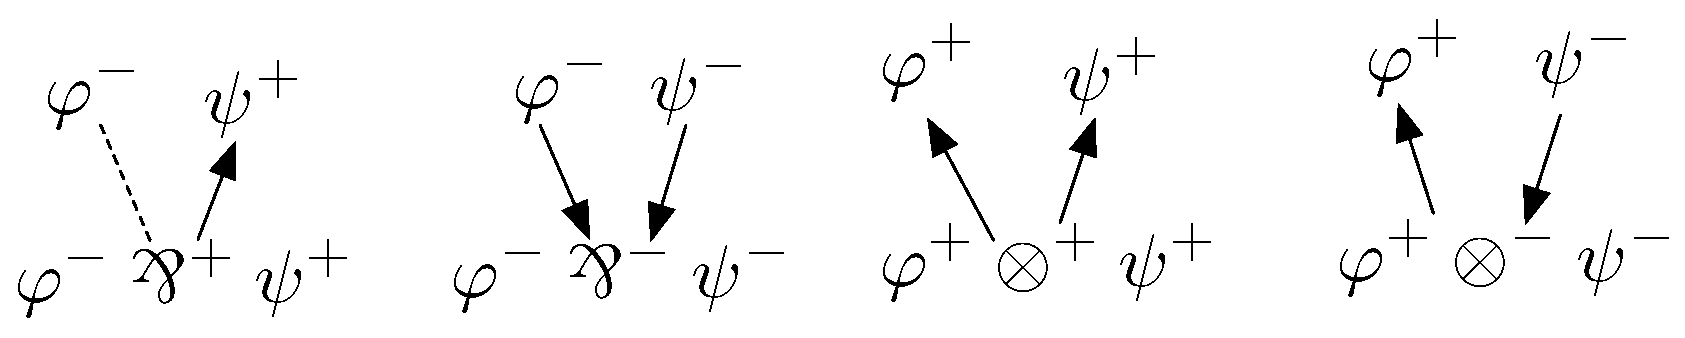
\includegraphics[scale=0.4]{rules-original.eps}
 \end{center}
For brevity, we sometimes write only the top connectives of labeling
formulae.
In that case, these branching nodes above are denoted like this.
 \begin{center} %rules
  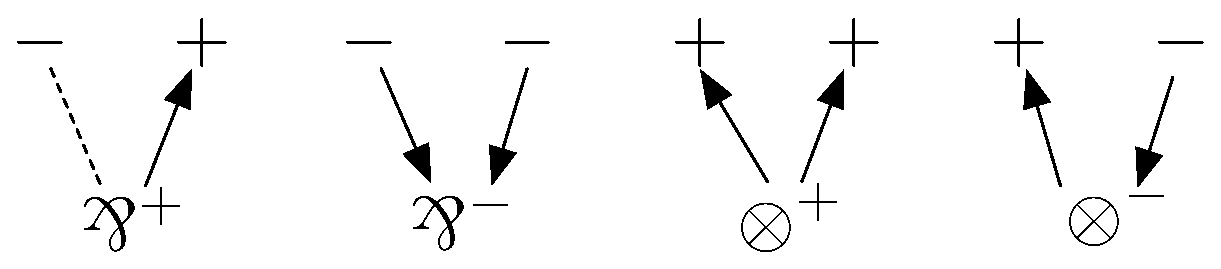
\includegraphics[scale=0.4]{rules.eps}
 \end{center}
We call arrows with upward (resp. downward) signs
\textit{up-edges}\index{up-edge}
(resp. \textit{down-edges}\index{down-edge}).
The \textit{dashed child}\index{dashed child}
of a $\parr^+$ node~$p$ is the node which the dashed
line from $p$ reaches.
The branching nodes labelled by $\parr^+, \parr^-, \otimes^+$ and
$\otimes^-$ are called \textit{operator nodes}.

When we add axiom edges and $\bot$-branches (shown below)
to the other operator nodes (shown above)
we obtain an \textit{essential net}\index{essential net} of $\phi$.
Due to the arbitrariness of choosing axiom edges and $\bot$-branches,
there are possibly multiple essential nets for a formula%
\footnote{\citet{murawski2003} restricts the class of formulae to linearly balanced
formulae so that the essential net is uniquely determined.}.
 \begin{center}
  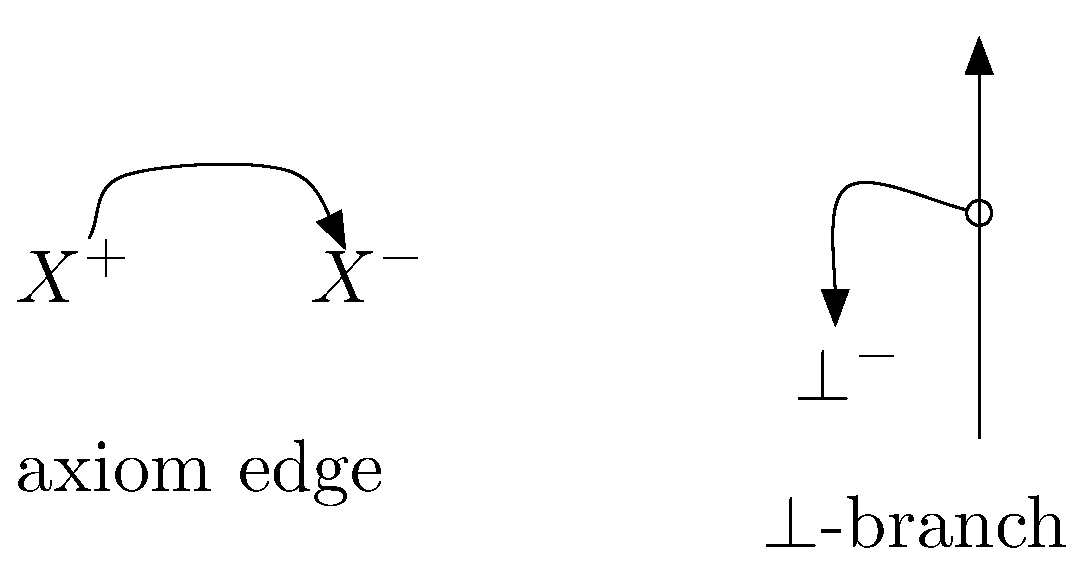
\includegraphics[scale=0.4]{axiom-cut.eps}
 \end{center}

 \begin{example}[An essential net of the Amida axiom] \label{essential-amida}
  Here is one of the essential nets of
  the Amida axiom $(X^-\parr^+Y^+)\otimes^+(Y^-\parr^+ X^+)$.
   \begin{center}
    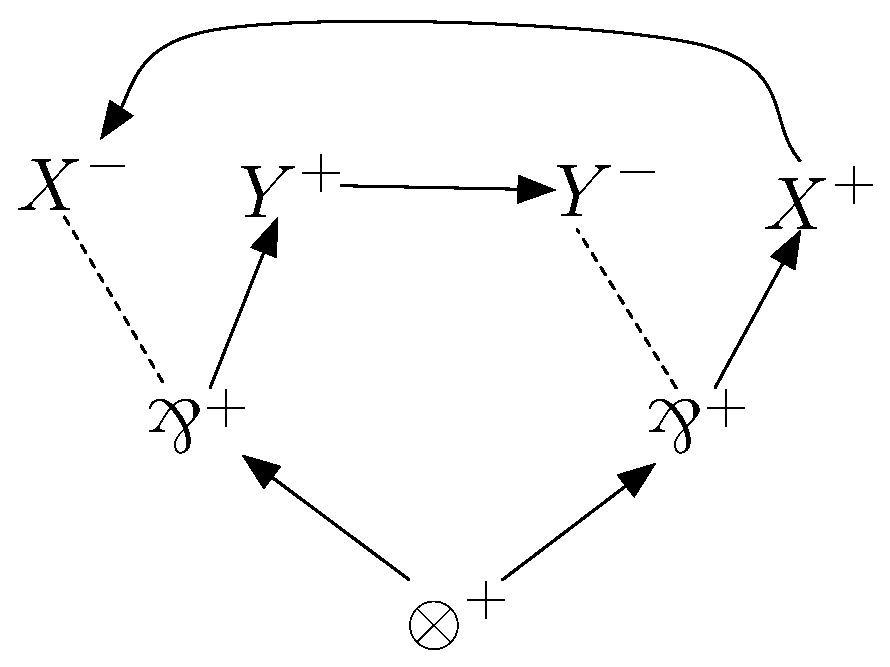
\includegraphics[scale=0.4]{amida-essential.eps}
   \end{center}
 \end{example}
 However, the essential net in \thref{essential-amida} is rejected by
 the following correctness criterion.
  \begin{definition}[Correct essential nets]
   A \textit{correct essential net}\index{correct essential
   net}\index{essential net!correct} is an essential net satisfying all
   these conditions:
\begin{enumerate}
 \item Any node labelled with $X^+$ (resp. $Y^-$) is connected to a
       unique node labelled with $X^-$ (resp. $Y^+$).
       Any leaf labelled with $\bot^-$ is connected to a $\bot$-branch.
       $\one^+$ is not connected to anything above itself;
 \item the directed graph formed by up-edge, down-edge, axiom edges and
       $\bot$-branches is acyclic;
 \item \label{conditionL}
       for every $\parr^+$-node~$p$, every path\footnote{A path must
       follow solid edges according to the direction.  Dashed edges are
       not directed and they are not contained in paths.}
       from the root that reaches
       $p$'s dashed child also passes through $p$.
\end{enumerate}
  \end{definition}
The essential net in Example~\ref{essential-amida} is not correct for
condition~\ref{conditionL}.  Actually, the Amida axiom does not have
any correct essential net.  IMLL sequent calculus has the subformula
property so that we can confirm that the Amida axiom is not provable in IMLL.

 \begin{theorem}[Essential nets for
  IMLL by~\citet{lamarche2008,murawski2003}]
  \label{essential-ok}
  An IMLL formula~$\phi$ is provable in IMLL iff there exists a correct essential net
  of $\phi$.
 \end{theorem}
 \begin{proof}
  The left to right is relatively easy.  For the other way around,
  \citet{lamarche2008} uses a common technique of decomposing an
  essential net from the bottom.
  \citet{murawski2003} chose to reduce the problem to sequents of special forms
  called regular.
 \end{proof}

 Actually, \citet{lamarche2008} also considers the cut rule\footnote{As well as
 additive operators and exponentials.} in essential nets, thus
 we can include the following general axioms (as macros) and cuts (as
 primitives) and still use \thref{essential-ok}:
 \begin{center}
  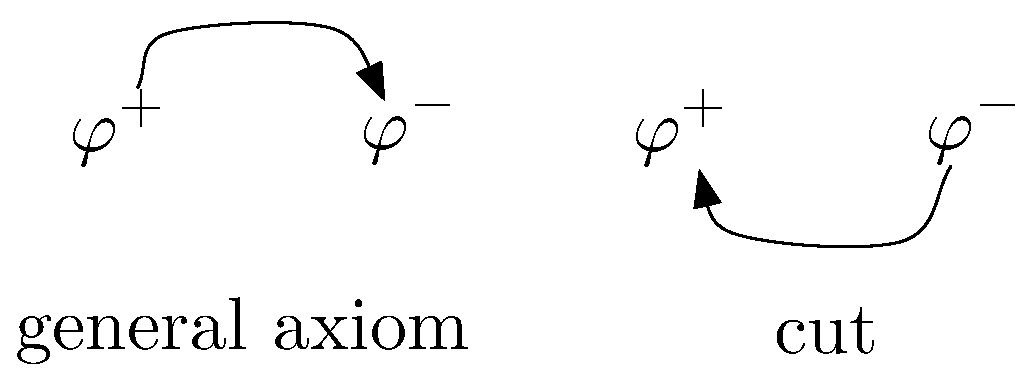
\includegraphics[scale=0.4]{general-axiom-cut.eps}\enspace.
 \end{center}

\subsection{The Amida Nets}

 \begin{definition}[The Amida nets]
  \label{def:amidanets}
For a hypersequent~$\hyper$,
\textit{Amida nets}\index{Amida nets} of $\hyper$ are inductively
  defined by the following three clauses:
\begin{itemize}
 \item an essential net of $\hyper$ is an Amida net of $\hyper$;
 \item for an Amida net of $\hyper$ with two different\footnote{The two edges can
       be connected by a new edge as long as they are different; their
       relative positions do not matter.} up-edges,
	\begin{center}
	 % twoedges
	 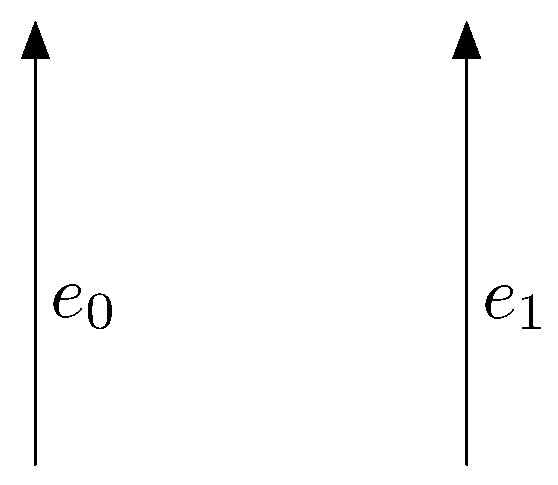
\includegraphics[scale=0.4]{twoedges.eps}
	\end{center}
       replacing these with
	\begin{center}
	 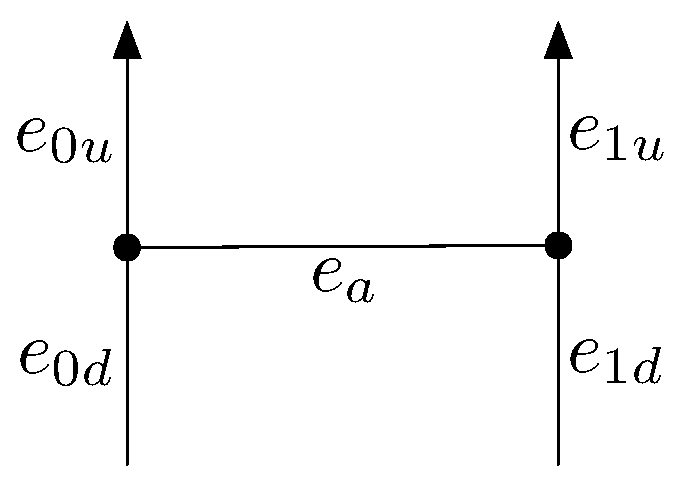
\includegraphics[scale=0.4]{twoedges_amida.eps}
	\end{center}
       yields an Amida net of $\hyper$,
       where the above component has two paths $e_{0d} e_a e_{1u}$
       and $e_{1d} e_a e_{0u}$;
 \item for an Amida net of $\hyper$ with an up-edge,
	\begin{center}
	 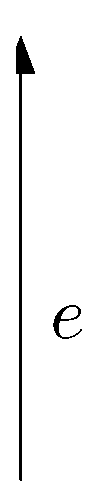
\includegraphics[scale=0.4]{oneedge.eps}
	\end{center}
       replacing this with
	\begin{center}
	 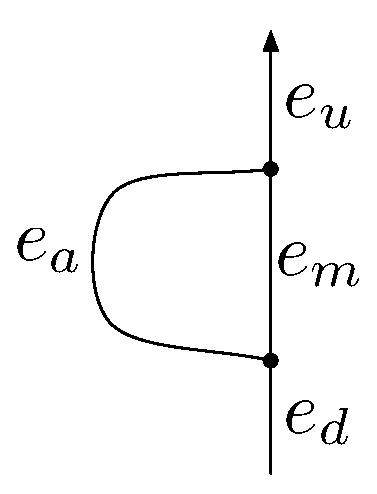
\includegraphics[scale=0.4]{oneedge_amida.eps}
	\end{center}
       yields an Amida net of $\hyper$,
       where the above component has
       one finite path $e_de_ae_u$
       and one infinite path $\cdots e_m e_a e_m e_a \cdots$.
\end{itemize}
 \end{definition}
 In these clauses, we call the edges labelled~$e_a$ the \textit{Amida
 edges}\index{edge!Amida}\index{Amida edge}.

 \begin{definition}[Correct Amida nets]
  A \textit{correct}\index{Amida net!correct}\index{net!correct
  Amida}\index{correct Amida net}
  Amida net is an Amida net satisfying the three conditions
  in Definition~\ref{def:amidanets}.
 \end{definition}

 The Amida edge is not merely a crossing of up-edges.
 See the difference between
 \begin{center}
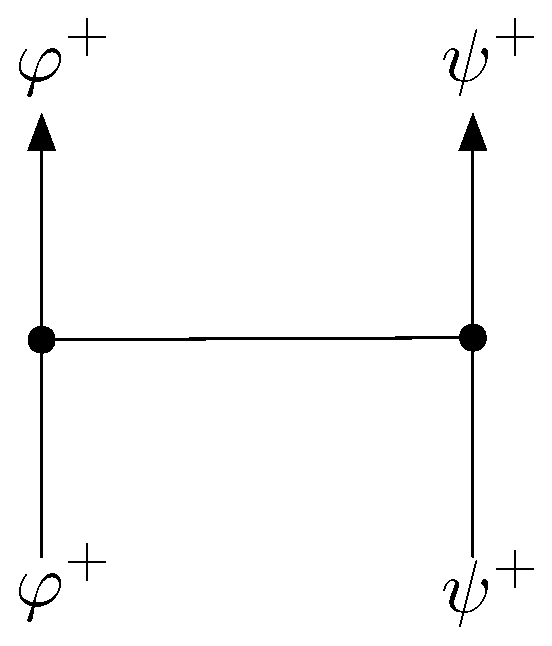
\includegraphics[scale=0.4]{twoedges_amida_without_label.eps}
 \end{center}
and
 \begin{center}

\includegraphics[scale=0.4]{crossing.eps}\enspace.
 \end{center}
The difference is the labels at the bottom.
Although Amida edges cross the paths,
they do not transfer labels.
This difference of labels makes Amida nets validate the Amida axiom.
 \begin{example}[A correct Amida net for the Amida axiom]
  Here is a correct Amida net for the Amida axiom $(X\limp Y)\otimes(Y\limp X)$.
   \begin{center}
    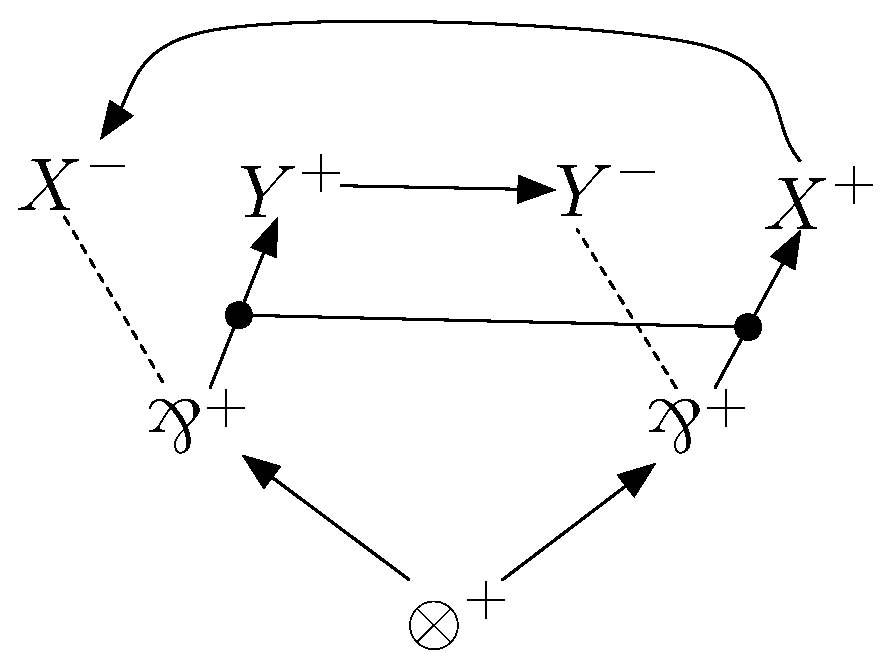
\includegraphics[scale=0.4]{amida-axiom.eps}
   \end{center}
  In terms of the set of paths, the above Amida net is equivalent to the
  following correct essential net for $(X\limp X)\otimes (Y\limp Y)$.
   \begin{center}
    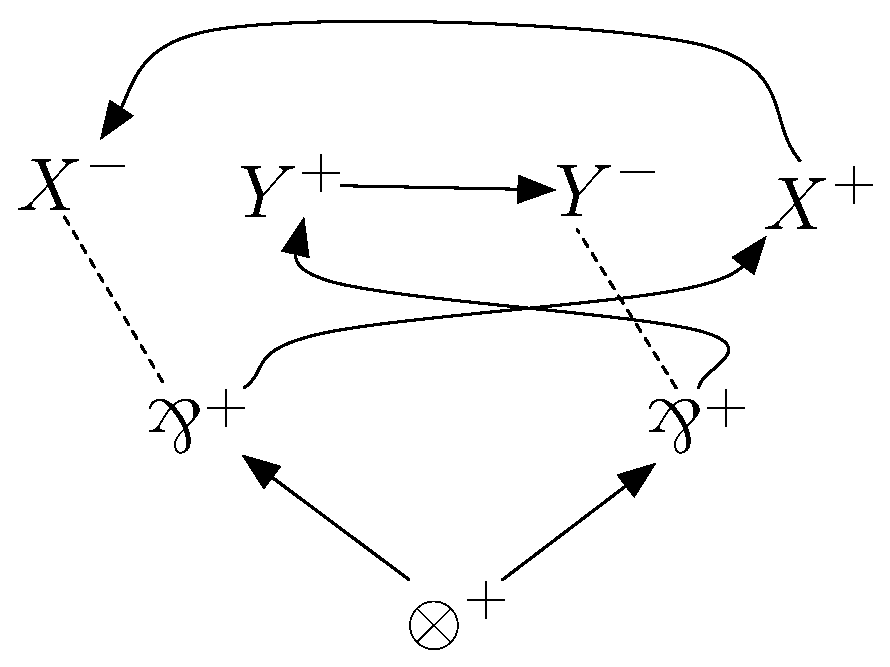
\includegraphics[scale=0.4]{amida-axiom-cross.eps}
   \end{center}
 \end{example}

\subsection{Soundness and Completeness of Amida nets}

 \begin{theorem}[Completeness of Amida nets]
  \label{amida-net-complete}
  If a hypersequent $\hyper$ is derivable,
  there is a correct Amida net for $\hyper$.
 \end{theorem}
 \begin{proof}
  Inductively on hypersequent derivations.
  The Sync rule is translated into a crossing with an Amida edge:
   \begin{center}
    \AxiomC{$\G\tr\phi\hmid\D\tr\psi$}
    \UnaryInfC{$\G\tr\psi\hmid\D\tr\phi$}
    \DisplayProof
    \quad
    $\mapsto$
    \quad
    $\vcenter{\hbox{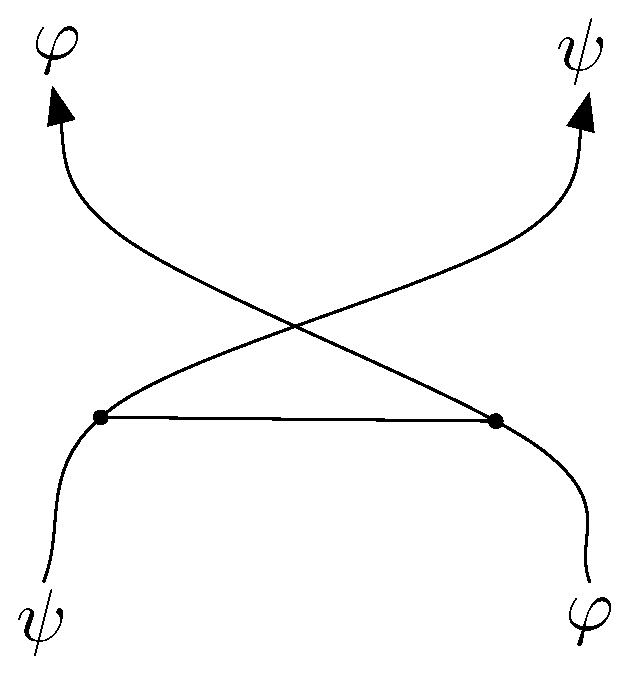
\includegraphics[scale=0.4]{sync-trans.eps}}}$
   \end{center}
  where the crossing exchanges the formulae and the Amida edge keeps the
  path connections vertically straight.
 \end{proof}
 \begin{theorem}[Soundness of Amida nets]
  If there is a correct Amida net for a hypersequent~$\hyper$, then
  $\hyper$ is derivable.
 \end{theorem}
 \begin{proof}
  From a correct Amida net, first we move the Amida edges upwards
  until they are just below axiom edges.
The moves are as follows.
 \begin{center}
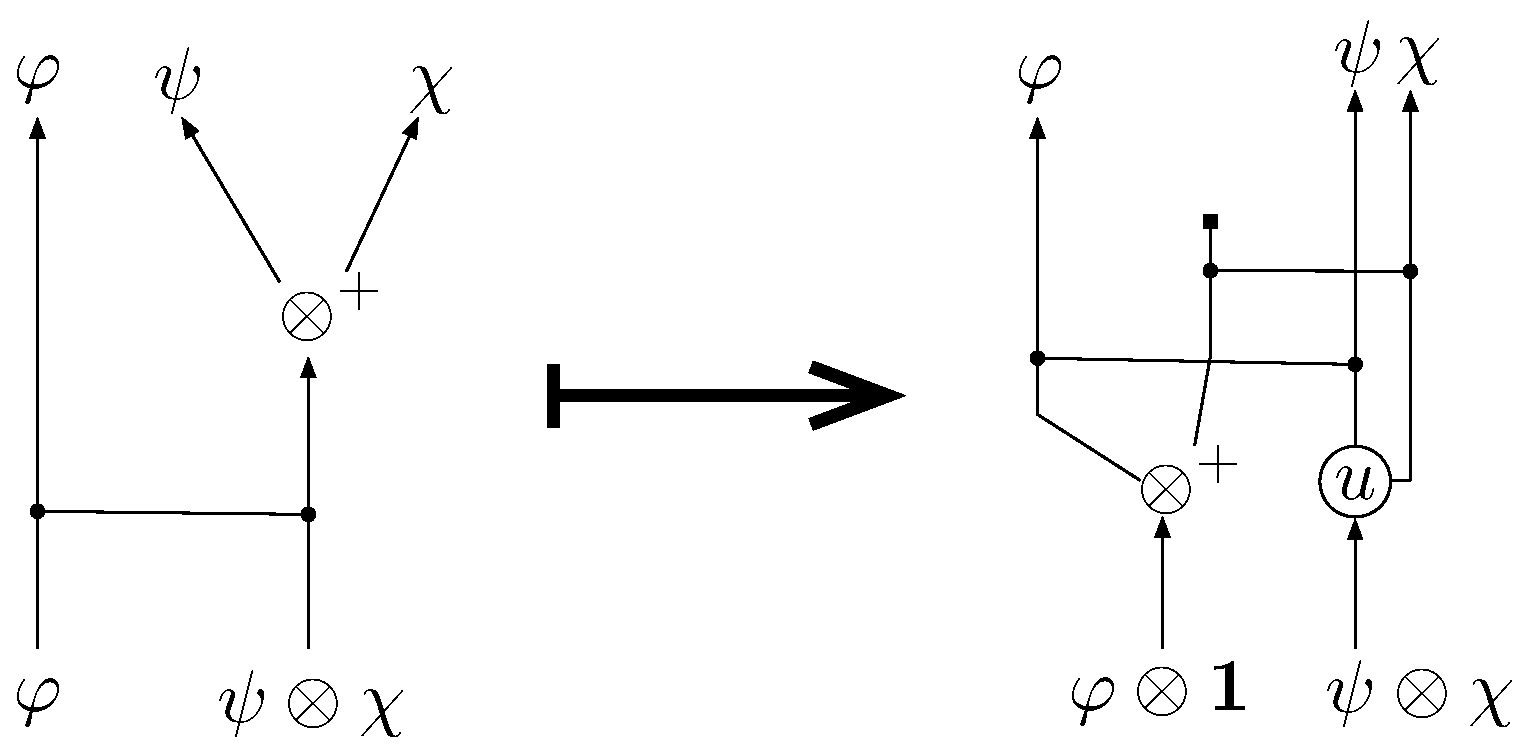
\includegraphics[scale=0.4]{tensor-move.eps}
\vskip 3cm
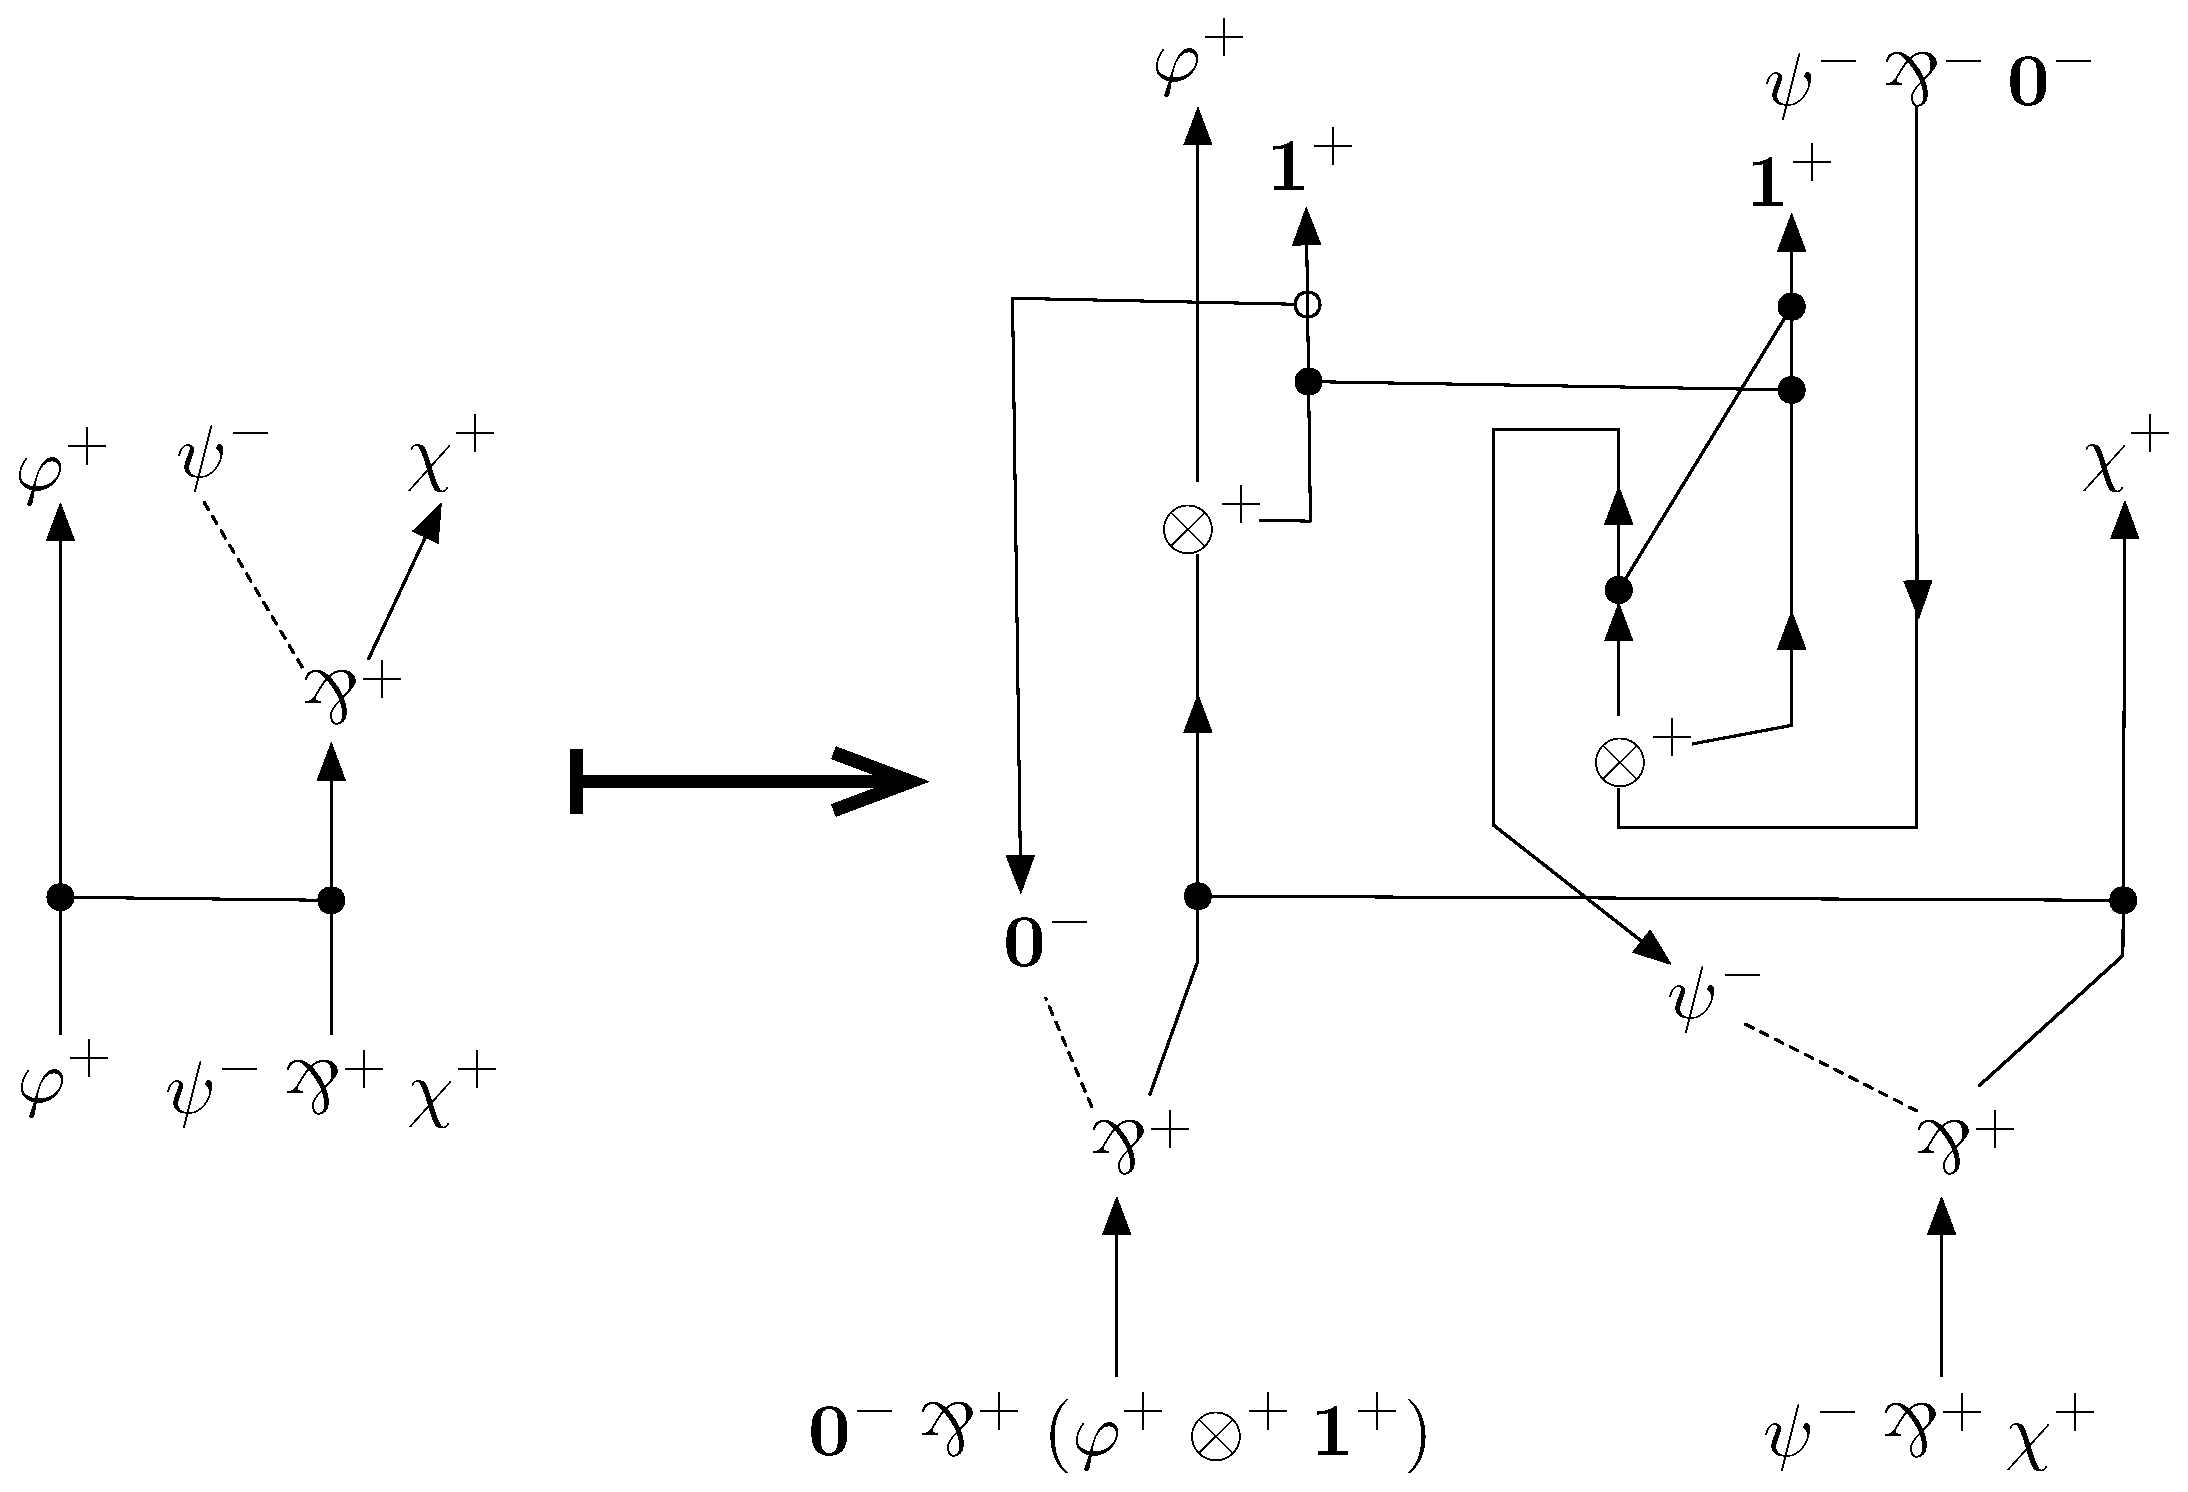
\includegraphics[scale=0.35]{parr-move.eps}
 \end{center}
These translations have two properties.
\begin{enumerate}
 \item When the original (contained in a larger picture)
       is a correct Amida net, the translation (contained in the same
       larger picture) is also a correct Amida net.
 \item The end nodes of the translation corresponds to the end nodes of
       the original, and the corresponding end nodes have the same label
       (up to logical equivalence in IMLL).  In case of $\otimes$
       translation, $\phi$ and
       $\phi\otimes \one$ are logically equivalent because $\one$ is the
       unit of $\otimes$.
       In case of $\parr$ translation, $\phi$ and $\bot\parr \phi$ are
       logically equivalent because $\bot$ is the unit of $\parr$.
\end{enumerate}
For checking the first condition, it is enough to follow the paths
(crossing all Amida edges).
For the second condition, it is enough to follow the vertical edges
ignoring the Amida edges and $\bot$-branches.

The $\otimes$ move introduces Amida edges only above the branching rules.
Although the $\parr$ move introduces an Amida edge below a
branching rule, that branching rule is of $\otimes$ nature.
Also, the $\parr$ move introduces an Amida edge below $\psi$-axiom link,
which is actually a macro.  So we have to continue applying the
translation moves in the macro.  However, Since $\psi$ is a strictly
smaller subformula of $\psi\parr\chi$, this does not cause infinite
recursion.

Then, by these translation moves,
the whole Amida net is decomposed vertically into three layers.
At the top, there is a layer with only axiom edges.
In the middle, there is a layer with only vertical edges and Amida
edges.
At the bottom, there is a layer which contains only ordinary
essential net nodes.

Since the middle layer is an Amida lottery, it defines a permutation.
That permutation can be expressed as a product of transpositions, so
that
the original Amida lottery is equivalent to an encoding of a
  hypersequent derivation
that consists of only Sync rules.

After we encode the top and the middle layer into a hypersequent
derivation, encoding the bottom layer
can be done in the same way as Lamarche's approach~\citep{lamarche2008}.
\end{proof}

We wonder whether it is possible to add Amida edges to
the IMALL$^-$ essential nets following
\citet{lamarche2008}.
The additives are notoriously difficult for proof nets and we do not
expect the combination of additive connectives and Amida edges can be
treated in a straightforward way.

\section{Related Work}

\subsection{Analytic Calculus for Abelian Logic}

\citet{metcalfe2002} gave a labelled sequent calculus for Abelian logic.
Some years later,
\citet{metcalfe2006} gave a hypersequent caluclus for Abelian logic and
proved cut-elimination theorem for the hypersequent calculus.
His formulation is different from ours because Metcalfe's system does
not use conjunctive hypersequents.  He sticks to the traditional
hypersequent formulation where components are interpreted disjunctively.
The paper \citep{metcalfe2006} is informative about some logics weaker
than Abelian logic so that there might be a hint of getting a
hyper-lambda calculi for these weaker logics.

Before \citet{metcalfe2002},
\citet{shirahata} studied the multiplicative fragment of Abelian logic,
which he called CMLL (compact multiplicative linear logic).
He gave a categorical semantics for the proofs of a sequent calculus
presentation of CMLL and then proved
that the cut-elimination procedure of
the sequent calculus preserves the semantics.
Since our Amida net presentation also gives a non-degenerate semantics
for the same logic, we speculate that Amida nets provide a suitable
presentation for morphisms of compact closed categories.
Remarkably,
\citet{shirahata} also noted that addition of infinite additives yields
inconsistency
although he did not notice his CMLL is identical to the multiplicative
fragment of Abelian logic\footnote{
\citet{expanding} already pointed out
the fact that \citet{shirahata} and
\citet{metcalfe2002} studied the same logic.}.
He also noted that addition of finite additives yields a counter-example
of cut-elimination, which we will note in Subsection~\ref{amida-cut}.

\subsection{Linear Logic and Session Types}

Session types~\citep{interaction,honda-session} apperaed in this chapter.
Session types aim at typing channels and processes in $\pi$-calculus so
that the process execution is deterministic and not ending in deadlock.
In general, session type systems are not based on a well-known logic.
However, there are recent developments on encoding session types into
linear type systems.

\subsubsection{Kobayashi-Pierce-Turner's Type System}

\citet{kobayashi-pierce-turner} developed a type system for the
$\pi$-calculus processes.
Similarly to the type system presented here,
their type system can specify
types of communication contents through a name and
how many times a name can be used.
In some sense,
that type system is more flexible than the one shown in this chapter.
First, their type system allows a liberal typing on a channel so
that the channel can be used for any number of times.
Second, their type system can type replicated processes.
Third, their type system allows
weakening~\citep[Lemma~3.2]{kobayashi-pierce-turner}.
In other respects,
the type system in \citep{kobayashi-pierce-turner} is less expressible.
That type system does not have lambda abstractions.
Also, in contrast to our type system,
it is impossible to substitute a free variable with a process in that
type system.
This is related to the fact that in their type system,
a sequent contains types on the left side but not on the right side.
Since there are no types on the right side, their sequent is hard to
interpret logically.

\subsubsection{Caires and Pfenning's Typing System}
\label{pfenning}

\citet{pfenning2010} provide a type system for a fragment of $\pi$-calculus.
Their type system imposes a discipline stronger
than necessary to provide deadlock freedom.
For example, this escrowing process $P$ below is not typable in their type
system:
\[
 P = \sendterm x y{\recvterm x a {\recvterm y b {\sendterm x b
 {\sendterm y a 0}}}}\enspace.
\]
The process first emits a channel~$y$ through channel~$x$ and then
takes inputs from $x$ and $y$ and outputs them respectively to $y$ and $x$.
Following the informal description of types by \citet{pfenning2010},
the process~$P$ should be typable as
\[
 \vdash P::x:(A\limp B)\otimes(B\limp A)\enspace.
\]
However, such typing is not possible because $(A\limp B)\otimes (B\limp
A)$ is not a theorem of dual intuitionistic linear logic (DILL), which
their type system
is based on.
In our type system, the following sequent is derivable
\begin{align*}
&
\tj{x}{\sendtype{(\sendtype{B}{\recvtype{A}\terminate})}{\recvtype B
{\sendtype A \terminate}}}
\tr\\
&\tj{
\nu(\tj{y}{\sendtype B{\recvtype A \terminate}}).
{\sendterm x{y_L}{\recvterm x a {\recvterm {y_R} b {\sendterm x b {\sendterm
{y_R} a {\ign{x,y}0}}}}}}
}{\one}
\end{align*}
The resulting sequent indicates that the process is typable with one
open channel~$x$ that first emits
a channel that one can send~$B$ to and receive~$A$ from, second receives a
value of $B$ and
finally sends a value of $A$.
This example shows that our type system can type some terms that
the type system in \citet{pfenning2010} cannot.

The most complicated example in \citet{pfenning2010} involves a drink server.
 \begin{example}[Drink server from \citet{pfenning2010} in Amida
  calculus]
  \begin{align*}
   ServerProto &= (N\limp I \limp (N\otimes \one))\with (N\limp( I
  \otimes \one)) \\
   &= (\sendtype N {\sendtype { I} {\recvtype N \terminate}}) \with
   (\sendtype N {\recvtype { I} \one})
  \end{align*}
  $N$ stands for the type of strings and $I$ stands for the type of
  integers, but following \citet{pfenning2010}, we identify both $N$ and
  $I$ with $\one$.  Below, $SP$ abbreviates $ServerProto$.
  Here is the process of the server, that serves one client and
  terminates.\\
  \[
   Serv = \lpair{\recvterm s {pn} {\recvterm s {cn} {\sendterm s {rc}
  {\ign {pn, cn, s} 0}}}
  ,\quad
  \recvterm s {pn} {\sendterm s {pr} {\ign{s,pn} 0}}
  }
  \]
  We can derive a sequent $\tj{s}{\overline{SP}}\tr\tj{Serv}\one$.

  Here is one client:
  \begin{center}
   \AxiomC{}
   \UnaryInfC{$\tr\tj{0}\one$}
   \UnaryInfC{$\tj{s}{\terminate}\tr\tj{\ign s 0}\one$}
   \UnaryInfC{$\tj{s}{\terminate},
   \tj{pr}{I}\tr\tj{\ign{pr,s} 0}\one$}
   \UnaryInfC{
   $ \tj{s}{\recvtype {I} {\terminate}} \tr\tj{
   \recvterm s {pr} {\ign{pr,s} 0}
   }{\one}$
   }
   \AxiomC{}
   \UnaryInfC{$ \tr\tj{tea}{N} $}
   \BinaryInfC{
   $ \tj{s}{\sendtype N {\recvtype {I} \terminate}} \tr\tj{
   \sendterm s {tea}
   {\recvterm s {pr} {\ign{pr,s} 0}}
   }{\one}$
   }
   \UnaryInfC{
   $ \tj{s}{ServerProto} \tr\tj{
   \letin s {\lpair{\_, s}} {
   \sendterm s {tea}
   {\recvterm s {pr} {\ign{pr,s} 0}}}
   }{\one}$
   }
   \DisplayProof
  \end{center}
  In words, the client first chooses the server's second protocol, which
  is price quoting, and asks the price of the tea, receives the price
  and terminates.

  We can combine the server with this client.
  However, since the Amida calculus lacks the exponential modality, Amida calculus
  cannot type any term with $!ServerProto$, which the type system of
  Caires and Pfenning can~\citep{pfenning2010}.
  In order to do that, we might want to tolerate inconsistency and
  add $\mu$ and $\nu$ operators
  from the modal $\mu$-calculus, like \citet{mumall} did, and express
  $!ServerProto$ as $\nu X. (SeverProto\otimes X)$.
 \end{example}

\subsubsection{Wadler's Encoding}

\citet{wadler2012propositions} gave a type system for a process
calculus based on classical linear logic.
Although the setting is classical, the idea is more or less the same as
\citet{pfenning2010}.
Wadler's type system cannot type the escrowing process above.
Worse, the definition of processes by \citet{wadler2012propositions}
does not recognize the escrowing process
\[
 \sendterm x y{\recvterm x a {\recvterm y b {\sendterm x b {\sendterm y
 a 0}}}}
\]
as a process at all.
His grammar requires the output construction to be used in the form
\[
 \sendterm x y {(P\mid Q)}
\]
where $x$ is bound in $Q$ but not in $P$ and $y$ is bound in $P$ but not
in $Q$.
Of course, there is a way to escape the above restriction by making $P$
and $Q$ communicate, but that option is prohibited by the typing rules.

\citet{wadler2012propositions} uses classical linear logic rather than
intuitionistic linear
logic.
He justifies the choice for ``greater simplicity and symmetry.''
In terms of provability, the shift from intuitionistic to classical
linear logic will not make any difference.  However, in terms of proof nets,
one difficulty looms.  In classical multiplicative linear logic,
adding the Amida edges to proof nets seems harder than the intuitionistic case
because classical MLL proof nets have no direction on edges.
After a path crosses an Amida edge, the author has no idea which
direction the path should continue; one plausible solution is doing
path-tracking in parallel and make these path-tracking processes synchronize
on Amida edges.

That said,
Wadler's type system is similar to ours;
our abbreviations are largely taken from Wadler's translations.

\subsubsection{Giunti and Vasconcelos's Type System}

\citet{giunti2010} give a type system for the pi calculus with the type
preservation theorem. Their type system is
extremely similar to our type system.
They say ``the goal of this work is to equip types with a constructor
able to denote the two ends of a same
channel''~\citep[Introduction]{giunti2010}.
One of their typing rules
 \begin{center}
  \AxiomC{$\G,x\colon(S,\overline S)\tr P$}
  \UnaryInfC{$\G\tr(\nu x)P$}
  \DisplayProof
 \end{center}
 is similar to a rule in \thref{typing_connection}
 \begin{center}
  \AxiomC   {$\hypert\hmid
  \G,\tj{x}{\phi^\sim},\tj{y}{\overline{\phi^\sim}}\tr\tj t \psi$}
  \UnaryInfC{$\hypert\hmid
  \G\tr\tj{\nu\tj{x}{\phi^\sim}.t[x_L/x][x_R/y]}{\psi}$}
  \DisplayProof\enspace.
 \end{center}
 In many cases, the Curry-Howard correspondence is followed from the logical world
 to the programming world: for already known logics, new lambda
 calculi are invented (e.g.~\citep{lambdamu,murphy,abe2007}).
 However, in our case, it seems that we have just
 found a connection between
 an already known logic called Abelian logic and an already known
 typing discipline invented by \citet{giunti2010}.
 It will be worthwhile to compare their system with our type system closely.

 \subsection{Join Calculus}

 The join calculus~\citep{join} is a process calculus, which is used as a basis for a
 language JoCaml~\citep{fournet2002jocaml}.
 An implicit typing system~\citep{fournet1997} allowed the join calculus
 to be successfully merged with an ML family language OCaml, but the
 type system does not guarantee determinacy or ensure that all messages
 are consumed.

 \subsection{Continuations}
 The eval-subst rule enables an
 evaluation $\co c[C[cv]]\eval v$, which
 reminds us of the call-with-current-continuation
 primitive~\citep{rees1986} and shift/reset primitives~\citep{danvy1990,asai2007}.
 The appearance of these classical type system primitives is not
 surprising because Abelian logic validates $((p\limp q)\limp q)\limp p$,
 which is a stronger form of the double negation elimination.
 Possibly we could use the technique of \citet{asai2007} to analyze
 the Amida calculus with eval-subst rule.

 \subsection{Logic Programming}

 There are at least two ways to interpret logics computationally.
 One is proof reduction, which is represented by $\lambda$-calculi.
 The other is proof searching.
 We have investigated the Amida calculus, which embodies the proof reduction
 approach to the Amida axiom.
 Then what implication does
 The Amida axiom have in
 the proof searching approach?
 Let us cite an example from \citet[A.2]{kobayashi-yonezawa}:
 \begin{quote}
  Consumption of a message $m$ by a process $m\limp B$ is represented by
  the following deduction:
  \[
   (m\otimes(m\limp B)\otimes C)\limp (B\otimes C)
  \]
  where $C$ can be considered as other processes and messages, or an environment.
 \end{quote}
 Using the Amida axiom,
 the inverse
 \[
  (B\otimes C)\limp (m\otimes (m\limp B))\otimes C
 \]
 is derivable.
 This suggests that the Amida axiom states that some
 computation is reversible in the context of proof searching.
 We suspect that this can be
 useful within the realm of reversible computation~\citep{revcon}.

\section{Discussion}

% \subsection{Categorical Considerations}
% One might want to ask whether we can model the logic with
% a symmetric monoidal closed
% category~\citep{blute2004category}%
% % \footnote{Abelian category must have a
% % zero object and if we can model Abelian logic with Abelian category,
% % the logic must have no theorems or all formulae are
% % theorems.}
%   with identified isomorphisms
% $\sigma_{ABCD}\colon (A\limp B)\otimes (C\limp D)\rightarrow (A\limp D) \otimes
%  (C\limp B)$, with naturality conditions.
%  Before considering equality among morphisms,
%  we know there is a non-trivial example.
%   \begin{example}[Integer Model of {\citep[p.~107]{residuated}}]
%    \label{smcc}
%    The preorder formed by objects as integers and morphisms as the usual
%    order among integers~$\le$
%    forms a symmetric monoidal closed category with swaps
%    when we interpret $\otimes$ as addition and
%    $m \limp n$ as $n-m$.
%   \end{example}
%   On the other hand,
%   if we take another formulation requiring natural isomorphisms
%   $\mathcal C(C,A)\times\mathcal C(D,B) \cong \mathcal C(D,A)\times
%   \mathcal C{(C,B)}$,
%   only singletons can be preorder models because $\tuple{id_A,id_B}$ is
%   mapped to $\tuple{f,g}$ where $f\colon A\rightarrow B$ and $g\colon
%   B\rightarrow A$ for any two objects $A$ and $B$.

% A straightforward reading of evaluation rules gives somewhat complicated
% equality conditions for morphisms.
% The condition says the following diagram commutes:
% \[
%    \begin{CD}
%     (A\limp B)\otimes (C\limp D) @>{d_{ABCD}}>> (A\otimes C)\limp(B\otimes D)\\
%     @VV{\sigma_{ABCD}}V @VV{id\limp s_{B,D}}V\\
%     (A\limp D)\otimes (C\limp B) @>{d_{ADCB}}>> (A\otimes C)\limp (D\otimes B)
%    \end{CD}
% \]
%  where $d_{ABCD}$ is induced by adjunction between $\otimes$ and $\limp$
%  from a morphism
%  $((A\limp B)\otimes (C\limp D))\otimes (A\otimes C)\rightarrow
%  (B\otimes D)$, which is provided by symmetric monoidal closed
%  properties.

%  Moreover, since $\phi^\ast \equiv \phi\limp\one$
%  has derivable sequents $\one \tr \phi^\ast \otimes \phi$
%  and $\phi\otimes\phi^\ast\tr \one$,
%  we can expect the semantics of $\phi^\ast$ to be the dual object of
%  that of $\phi$.
%  Indeed, checking one of the coherence condition of compact closedness
%  is evaluating the below typed term
%  \begin{center}
%   \AxiomC{$\tj t \phi$}
%   \AxiomC{}
%   \UnaryInfC{$\tr\tj{\ast}\one$}
%   \BinaryInfC{$\tr \tj t \phi \hmid \tr \tj \ast \one$}
%   \AxiomC{}
%   \UnaryInfC{$\tj x \phi \tr \tj x \phi$}
%   \AxiomC{}
%   \UnaryInfC{$\tr \tj \ast \one$}
%   \BinaryInfC{$\tj x \phi \tr \tj{cx}\one\hmid \tr \tj {\co c \ast}
%   \phi$}
%   \UnaryInfC{$\tj x \phi \tr \tj{cx} \one \hmid \tj{z}\one\tr \tj{\ign z
%   {\co c \ast}}\phi$}
%   \BinaryInfC{$\tr\tj t \phi\hmid \tj x \phi \tr \tj{cx}\one \hmid \tr
%   \tj{\ign \ast {\co c \ast}}\phi$}
%   \UnaryInfC{$\tr\tj{ct}\one \hmid \ign \ast {\co c \ast}\phi$}
%   \UnaryInfC{$\tr\tj{ct}\one \hmid \tj y \one \tr \tj {\ign y {\ign \ast
%   {\co c \ast}}} \phi$}
%   \UnaryInfC{$\tr \tj{\ign {ct}{\ign \ast {\co c \ast}}}\phi$}
%   \DisplayProof\enspace .
%  \end{center}
%  At least, if $t \eval v$ is derivable, $\ign {ct} {\ign \ast {\co c
%  \ast}}\eval v$ is also derivable.
%  \begin{center}
%   \AxiomC{$t\eval v$}
%   \AxiomC{}
%   \UnaryInfC{$\ast\eval \ast$}
%   \BinaryInfC{$t\eval v\hmid \ast\eval \ast$}
%   \UnaryInfC{$ct \eval \ast\hmid \co c\ast \eval v$}
%   \AxiomC{}
%   \UnaryInfC{$\ast\eval \ast$}
%   \BinaryInfC{$ct \eval \ast \hmid \ign \ast {\co c \ast} \eval v$}
%   \UnaryInfC{$\ign {ct} {\ign \ast {\co c \ast}}\eval v$}
%   \DisplayProof\enspace.
%  \end{center}
%  Showing the other direction is more
%  involved because of eval-subst rule, but the author expects the case
%  analysis on possible substitutions will succeed.

\subsection{Adding Agents, Recursions, \ldots}
Our type system has a drawback of having only finitely many processes.
We expect it straightforward to overcome this weak point by
adding recursions in our type system.
As a guidance we can take $\mu$MALL of \citet{mumall}.

It is tempting to add modalities representing agents
and then study the relationship with the
multiparty session types~\citep{sync-multi-session, async-multi-session}.
For that, intuitionistic epistemic logic by~\citet{hirailpar,hiraimaster}
will be useful.

In order to implement this lambda calculus as a programming language, we
need linear types.
If we seek a quick way of implementing our hyper-lambda calculus on top
of an existing ML family programming language, we have to choose the
existing language carefully.
For example, OCaml and Haskell uses intuitionistic type system so if we
use these languages naively, the Amida axiom makes the type system
inconsistent and some communication primitives can be thrown away,
leaving the peer deadlocked.
The uniqueness type of the programming language Clean~\citep{parle1991}
does not allow contraction, but the uniqueness type is
still not special enough because their type system allows weakening.

\subsection{Cut-Elimination}
\label{amida-cut}

In the Amida calculus, there is a hypersequent that
can be derived with the cut rule but not without cut rules.
For example,
$X, Y\tr X\hmid \tr Y$ can be derived with a cut rule application:
 \begin{center}
  \AxiomC{}
  \LL{Ax}
  \UnaryInfC{$Y\tr Y$}
  \AxiomC{}
  \LL{Ax}
  \UnaryInfC{$X\tr X$}
  \LL{$\limp$R}
  \UnaryInfC{$\tr X\limp X$}
  \LL{Merge}
  \BinaryInfC{$Y\tr Y\hmid \tr X\limp X$}
  \LL{Sync}
  \UnaryInfC{$Y\tr \underline{X\limp X}\hmid \tr Y$}
  \AxiomC{}
  \LL{Ax}
  \UnaryInfC{$X\tr X$}
  \AxiomC{}
  \LL{Ax}
  \UnaryInfC{$X\tr X$}
  \LL{Merge}
  \BinaryInfC{$X\tr X\hmid X\tr X$}
  \LL{$\limp$L}
  \UnaryInfC{$\underline{X\limp X}, X\tr X$}
  \LL{Cut}
  \BinaryInfC{$X,Y\tr X\hmid \tr Y$}
  \DisplayProof
 \end{center}
However, the conclusion is not derivable without the cut rule (as
confirmed by a simple proof searching).

Worse, it is easy to see that the prelinearity
$(\phi\limp\psi)\oplus(\psi\limp\phi)$ does not have a cut-free proof.
However,
since there is a cut-free deduction system for Abelian
logic~\citep{metcalfe2006},
we consider it natural to expect the same property for a suitable
extension of the Amida calculus, which would contain terms and reductions
corresponding to proof rules and proof reductions in the system of \citet{metcalfe2006}.

\subsection{The Problem with Excluded Middle}
\label{computational-meaning}

Since the Amida calculus characterizes Abelian logic,
there is a closed term~$t$ with the sequent $\tr\tj{t}{(X\limp \one)\oplus X}$
derivable.
We tried looking at one such term~$t$, but it involved channels
contained in lambda abstraction bodies and additive pairs.
Unfortunately, the closed lambda term does not choose left or right so
that it does not give a constructive justification to the excluded
middle.
Since the closed term~$t$ uses additive constructs, we expect the
multiplicative fragment to be much more explainable.

\subsection{Non-Commutative Version of the Amida Axiom}

Including the
the non-commutative version of the Amida axiom $(\phi/\psi)\otimes(\psi/\phi)$
to the full Lambek calculus turns out to be equivalent to
adding $(\psi\setminus\phi)\otimes(\phi\setminus\psi)$.
Algebraically speaking,
the set of equations of the form $(x/y)\cdot(y/x) = 1$ forms an
equational basis for $\mathsf{LG}$, the variety of lattice-ordered
groups.
In a lattice-ordered group,
$(x/y)\cdot (y/x) = (x \cdot y^{-1}) \cdot (y \cdot x^{-1}) = 1$.
On the other hand, assuming $(x/y)\cdot (y/x) = 1$, when we substitute 1
for $x$, we obtain $(1/y)\cdot (y/1) = 1$.
By the definition of residuation and the unit 1 of $\cdot$,
we have $(1/y)\cdot y = 1$, which forms an equational basis for the
variety of lattice-ordered groups \citep[Lemma~3.25]{residuated}.

\subsection{Program Specification and Verification}

Since the typing derivations of the Amida calculus can be interpreted as
proofs of Abelian logic, there is a possibility of specifying properties
of processes using (first-order) Abelian logic formulae and then
proving those properties using conjunctive hypersequents%
\footnote{When the author applied for Grant-in-Aid for JSPS Fellows
23-6978, the proposal included such a plan.  According to the proposal,
this research would proceed from finding a typed lambda calculus then to
developing a logic for proving properties of the obtained programming
language.}.
If that succeeds, the technique would be the first application of
Abelian logic in program verification.

\section{Conclusions}

We found a new axiomatization of Abelian logic, which can be
characterized by the Amida axiom
$(\phi\limp\psi)\otimes(\psi\limp\phi)$ on top of IMALL$^-$.
The axiomatization has an application for encoding process calculi and
session type systems.
As a technique, we used conjunctive hypersequents for the first time,
where components in a hypersequent are interpreted conjunctively rather
than disjunctively.
The resulting hyper-lambda calculus is somewhat hard to treat
theoretically.
If we need convergence or deadlock-freedom, we need the eval-subst rule in the evaluation rule
(Subsection~\ref{eval-subst}),
which poses a threat to type safety.
Moreover, there are some inhabited types like $\phi\oplus
(\phi\limp\one)$ and $(\phi\limp\psi)\oplus(\psi\limp\phi)$,
whose constructive justification is hard to see.
Plausibly, the situation can be remedied by extending the Amida net
approach treated in Section~\ref{sec:proofnets}.
